

\documentclass[final]{vutinfth} 

\usepackage{lmodern}        \usepackage[T1]{fontenc}    \usepackage[utf8]{inputenc} 

\usepackage{amsmath}    \usepackage{amssymb}    \usepackage{mathtools}  \usepackage{microtype}  \usepackage[inline]{enumitem} \usepackage{multirow}   \usepackage{booktabs}   \usepackage{subcaption} \usepackage[ruled,linesnumbered,algochapter]{algorithm2e} \usepackage[usenames,dvipsnames,table]{xcolor} \usepackage{nag}       \usepackage{todonotes} \usepackage{hyperref}  \usepackage{float}


\usepackage{listings, xcolor}

\definecolor{verylightgray}{rgb}{.97,.97,.97}

\lstdefinelanguage{Solidity}{
	keywords=[1]{anonymous, assembly, assert, balance, break, call, callcode, case, catch, class, constant, continue, constructor, contract, debugger, default, delegatecall, delete, do, else, emit, event, experimental, export, external, false, finally, for, function, gas, if, implements, import, in, indexed, instanceof, interface, internal, is, length, library, log0, log1, log2, log3, log4, memory, modifier, new, payable, pragma, private, protected, public, pure, push, require, return, returns, revert, selfdestruct, send, solidity, storage, struct, suicide, super, switch, then, this, throw, transfer, true, try, typeof, using, value, view, while, with, addmod, ecrecover, keccak256, mulmod, ripemd160, sha256, sha3}, keywordstyle=[1]\color{blue}\bfseries,
	keywords=[2]{address, bool, byte, bytes, bytes1, bytes2, bytes3, bytes4, bytes5, bytes6, bytes7, bytes8, bytes9, bytes10, bytes11, bytes12, bytes13, bytes14, bytes15, bytes16, bytes17, bytes18, bytes19, bytes20, bytes21, bytes22, bytes23, bytes24, bytes25, bytes26, bytes27, bytes28, bytes29, bytes30, bytes31, bytes32, enum, int, int8, int16, int24, int32, int40, int48, int56, int64, int72, int80, int88, int96, int104, int112, int120, int128, int136, int144, int152, int160, int168, int176, int184, int192, int200, int208, int216, int224, int232, int240, int248, int256, mapping, string, uint, uint8, uint16, uint24, uint32, uint40, uint48, uint56, uint64, uint72, uint80, uint88, uint96, uint104, uint112, uint120, uint128, uint136, uint144, uint152, uint160, uint168, uint176, uint184, uint192, uint200, uint208, uint216, uint224, uint232, uint240, uint248, uint256, var, void, ether, finney, szabo, wei, days, hours, minutes, seconds, weeks, years},	keywordstyle=[2]\color{teal}\bfseries,
	keywords=[3]{block, blockhash, coinbase, difficulty, gaslimit, number, timestamp, msg, data, gas, sender, sig, value, now, tx, gasprice, origin},	keywordstyle=[3]\color{violet}\bfseries,
	identifierstyle=\color{black},
	sensitive=false,
	comment=[l]{//},
	morecomment=[s]{/*}{*/},
	commentstyle=\color{gray}\ttfamily,
	stringstyle=\color{red}\ttfamily,
	morestring=[b]',
	morestring=[b]"
}

\lstset{
	language=Solidity,
	backgroundcolor=\color{verylightgray},
	extendedchars=true,
	basicstyle=\footnotesize\ttfamily,
	showstringspaces=false,
	showspaces=false,
	numbers=left,
	numberstyle=\footnotesize,
	numbersep=9pt,
	tabsize=2,
	breaklines=true,
	showtabs=false,
	captionpos=b
} \usepackage{refcount}
\usepackage{seqsplit}
\usepackage[acronym,toc,nonumberlist]{glossaries} \newcommand{\hash}[1]{{\ttfamily\seqsplit{#1}}}
\newcommand{\authorname}{Michael Etschbacher} \newcommand{\thesistitle}{Reducing the operation cost of a file fixity storage service on the Ethereum blockchain by utilizing pool testing strategies.} \hypersetup{
    pdfpagelayout   = TwoPageRight,           linkbordercolor = {Melon},                pdfauthor       = {\authorname},          pdftitle        = {\thesistitle},         pdfsubject      = {Subject},              pdfkeywords     = {a, list, of, keywords} }

\setpnumwidth{2.5em}        \setsecnumdepth{subsection} 

\nonzeroparskip             \setlength{\parindent}{0pt} 

\makeindex      \makenoidxglossaries \newacronym{eth}{ETH}{Ether}
\newacronym{gwei}{GWEI}{Gwei}
\newacronym{p}{p}{Prevalence of corruption}
\newacronym{k}{k}{Optimal Pool Size}
\newacronym{oais}{OAIS}{Open Archival Information System}
\newacronym{eff}{E(S)}{Efficiency of strategy S compared to individual testing}
\newacronym{cost-eff}{C(S)}{Cost-Efficiency of strategy S compared to individual testing}
\newacronym{op-cost}{T(S)}{Operation Cost of strategy S in gas}
\newacronym{cost}{C(S)}{Cost Efficiency of strategy S compared to individual testing}
\newacronym{count_op}{O(S)}{Number of operations needed with strategy S}
\newacronym{count_wr}{W(S)}{Number of cost relevant operations needed with strategy S}
\newacronym{count_re}{R(S)}{Number of data scrubbing operations needed with strategy S}
\newacronym{individual}{$S_{i}$}{Individual testing strategy}
\newacronym{two-stage}{$S_{h}$}{Two-stage-hierarchical pooling strategy}
\newacronym{cs}{$S_{cs}$}{context-sensitive pooling strategy}
\newacronym{evm}{EVM}{Ethereum Virtual Machine}
\newacronym{dlt}{DLT}{Distributed Ledger Technology}
\newacronym{dapp}{DAPP}{Decentralized Application}

\newglossaryentry{transaction}
{
  name={transaction},
  description={An Ethereum transaction refers to an action initiated by an account managed from a human, changes the state of the blockchain.}
}
\newglossaryentry{call}
{
  name={call},
  description={An Ethereum call refers to an interaction with a smart contract which does not change the state on the blockchain.}
}
\newglossaryentry{data-scrubbing}
{
  name={data-scrubbing},
  description={Data-scrubbing is an error correction technique which replaces corrupted object with copies.}
}
\newglossaryentry{history-forgery}
{
  name={history-forgery},
  description={The creation of false artifacts.}
} 

\setauthor{Bsc.}{\authorname}{}{male}
\setadvisor{Ao.univ.Prof. Dr.}{Andreas Rauber}{}{male}

\setregnumber{51828999}
\setdate{19}{05}{2022} \settitle{\thesistitle}{\thesistitle} 

\setthesis{master}
\setmasterdegree{dipl.} \setcurriculum{Data Science}{Data Science} 

\begin{document}

\frontmatter 

\addtitlepage{naustrian} \addtitlepage{english} \addstatementpage

\begin{kurzfassung}
In dieser Arbeit geht es darum die Datenintegrität eines Digitales Archives, in welchem Kulturgüter wie Bilder oder Texte archiviert sind, mit Hilfe von blockchain Technologie zu sichern. Ich verschaffe einen Überblick über digitale Archive und das Konzept von Vertrauen, Authentizität und Integrität von Daten in Archiven und eine Methode, um diese Konzepte zu stärken. In der modernen Zeit, in der das Fälschen und Manipulieren von Daten einfacher denn je ist, ist es umso wichtiger, das Vertrauen in öffentliche Einrichtungen wie Archive zu stärken.
Um die Datenintegrität zu gewährleisten, werden üblicherweise Kryptografische Verfahren angewandt, um sogenannte Fixitäts Informationen zu erstellen. Fixität ist ein Attribut eines digitalen Objekts, mit welchem validiert werden kann, dass ein Objekt über einen gewissen Zeitraum nicht manipuliert wurde. Auch wenn das Erstellen von Fixitäts Informationen (z.B. MD5, SHA256) relativ einfach ist, ist das Speichern von dessen umso schwerer, wenn Sie bedenken, dass jeder der diese ändern kann auch die zu Grunde liegenden Daten ändern kann.
Als Speichermedium für die Fixität stelle Ich in dieser Arbeit die Ethereum blockchain vor. Es wurde bereits gezeigt, dass die Ethereum blockchain geeignet ist, um Metadaten unveränderbar zu persistieren, jedoch sind die Kosten für eine Individuelle Strategie, in welcher die Metadaten jedes Objektes einzeln in der Blockchain persistiert werden, immens.
Um den Kosten entgegenzuwirken, werde Ich eine Pool-Testing-Strategie anwenden, in welcher mehrere digitale Objekte in einem Pool zusammengefasst werden. Somit wird die Anzahl an kostenpflichtigen Transaktionen auf der blockchain minimiert, wobei trotzdem die Effizienz gewahrt wird. Die Idee zu diesem Vorgehen stammt aus der derzeitigen Pandemie, in der die Testkapazitäten optimal genutzt werden müssen.
In der Evaluation berücksichtige Ich die verursachten Kosten und die Effizienz einer Pooling-Strategie im Vergleich zur individuellen Strategie. Ich zeige, anhand des OpenPreserve Format Korpusses, dass die Anzahl an benötigten Fixitäts Tests um das 2.25-Fache und die Kosten um das 5-Fache durch eine Pooling-Strategie reduziert werden können. Ich zeige zudem eine Kontext sensitive Pooling-Strategie, welche die Volatilität einzelner Dateiformate berücksichtigt und dadurch angepasste Poolgrößen anwendet. Die Kontext sensitive Methode ist ausbalancierter mit einer Testreduzierung um das 3.28-Fache und einer Kostenreduzierung um das 3.48-Fache.
Der Beitrag dieser Arbeit zu diesem Forschungsfeld ist die exakte Kostenberechnung eines dezentralen Fixitätsspeichers auf der Ethereum blockchain und zusätzlich eine Methode, um die Kosten eines solchen zu reduzieren.

 \end{kurzfassung}

\begin{abstract}
This work is about securing the data integrity of a digital archive, in which cultural assets such as images or text are stored, with the help of blockchain technology. I provide an overview of digital archives and the concepts of trust, authenticity, and integrity of data in archives and a method to strengthen these concepts. In a modern age, where falsifying and manipulating data is easier than ever, it is even more important to strengthen trust in public institutions.
To ensure data integrity, cryptographic methods are usually used to create so-called fixity information. Fixity is an attribute of a digital object that can be used to validate that an object has not been tampered with for a certain time interval. While generating fixity information (e.g., MD5, SHA256) is relatively easy, storing it is more difficult when you consider that anyone who can change it can also change the underlying data.
In this work, I present the Ethereum blockchain as a storage medium for the fixity information. It has already been shown that the Ethereum blockchain is suitable for persisting metadata in an unchangeable manner, but the costs for an individual strategy in which the metadata of each object is persisted individually in the blockchain are immense.
To counteract the costs, I utilize a pool testing strategy in which several digital objects are pooled. This minimizes the number of chargeable transactions on the blockchain while still maintaining efficiency. The idea for this approach stems from the ongoing pandemic, in which the test capacities must be used optimally.
In the evaluation, I consider the costs incurred and the efficiency of a pooling strategy compared to an individual strategy. I show, using the OpenPreserve format corpus, that the number of required fixity tests can be reduced by a factor of 2.25 and the cost by a factor of 5 by utilizing a pooling strategy. I also show a context-sensitive pooling strategy that considers the volatility of individual file formats and thus applies adjusted pool sizes. The context-sensitive method is more balanced with a test reduction of 3.28x and a cost reduction of 3.48x.
The contribution of this work to this research field is the exact cost computation of a decentralized fixity storage on the Ethereum blockchain and additionally a method to reduce the costs of such. \end{abstract}

\selectlanguage{english}

\tableofcontents 

\mainmatter

\chapter{Introduction}
\section{About Data Integrity}
Storing cultural heritage in digital archives offers malicious actors the possibility to manipulate the data and possibly forge history. Recent digital technologies make data manipulation more efficient, less costly, and more exact and there is a long history of forging history. 
In 1920 a photography was taken of Vladimir Lenin atop a platform speaking to a crowd. In the original photo, see Figure \ref{fig:f1}, Lenin's comrade Leon Trotsky can be seen standing beside the platform on Lenin's left side. When power struggles within the revolution forced Trotsky out of the party 7 years later, he was retouched out of the picture, see Figure \ref{fig:f2}, using paint, razors and airbrushes. Soviet photo artists altered the historical record by literally removing Trotsky from the pictures \cite[3]{hofer2005digital}.

\begin{figure}[t]\centering
    \begin{subfigure}{6cm}
    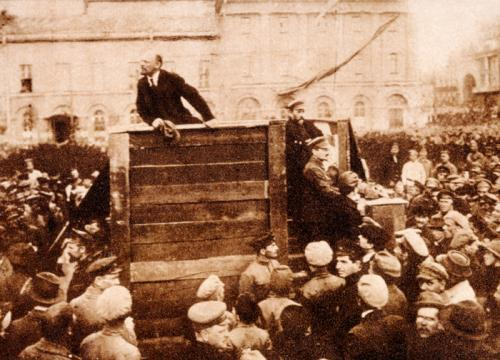
\includegraphics[width=\linewidth]{graphics/trotzki1.jpg}
    \caption{Original}\label{fig:f1}
    \end{subfigure}
    \qquad
    \begin{subfigure}{6cm}
    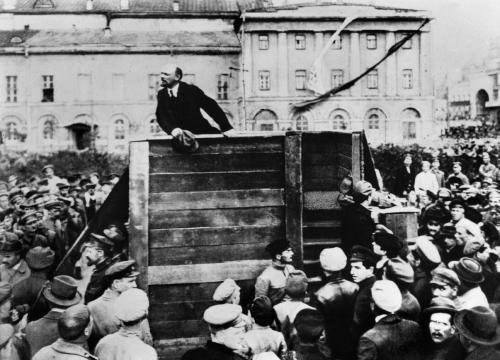
\includegraphics[width=\linewidth]{graphics/trotzki2.jpg}
    \caption{Retouched}
    \label{fig:f2}
    \end{subfigure}
    \caption{Catalog Images}
\end{figure}

Digital archives must earn the trust of current and future digital creators by developing a robust infrastructure and long-term preservation plans to demonstrate that the archive and its staff are trustworthy stewards of the digital materials in their care \cite[37]{kirschenbaum2010digital}. Digital objects can be corrupted easily, with or without fraudulent intent, and even without intent at all. Data corruption is usually detected by comparing cryptographic hashes, so-called fixity information, at different time intervals \cite[1]{de2014checking}. The object is seen as uncorrupted if the hash values are identical, since the smallest change to the object would alter the newly computed hash value immensely. 

\section{Research Problem}
Although generating fixity information (e.g., MD5, SHA256) is relatively easy, managing that information over time is harder. Consider that if an actor can change the fixity information, the actor can also tamper the underlying data \cite[35]{kirschenbaum2010digital}. Fixity information is usually stored in databases; object metadata records or alongside content, whereas this thesis utilizes the blockchain as a storage medium.
It is shown, that the Ethereum blockchain is suited for storage of metadata, such as provenance data or fixity information \cite[1]{collomosse2018archangel}.

Collomosse et al. (2018) and Sigwart et. al (2020) have shown that the Ethereum blockchain, developed by Buterin et. al (2013), can indeed be utilized to ensure data integrity, but there is a problem with that: the operation cost. The cost of storing a SHA256 values on the Ethereum blockchain is about \$8, which means the operation cost for an ingest of 10,000 objects costs about \$80,000.

\section{Research Goal}
This thesis proposes a way to reduce the operational cost of a blockchain-based fixity information storage by applying a pool testing strategy in which several digital objects are combined in a pool to form a hash list. The idea for this approach stems from the ongoing pandemic, in which the test capacities also must be used optimally.
\begin{quote}
Pool testing strategies build on testing a pooled sample from several patients: if the results from the pool test are negative, all patients in the pooled sample are declared not to have COVID-19; if the results of the pool are positive, each patient sample is tested individually. The pooled testing strategy is appealing, particularly when test availability is limited \cite[1]{cherif2020simulation}.
\end{quote}
This paradigm will be utilized in this thesis where the test specimen are cryptographic hashes, and the pool is hash list. With pooled testing, the goal is to reduce the amount of transactions, and therefore the cost by at least 50\%.

\section{Research Questions}
Based on the problem described above, the following research questions arise:

\textit{RQ1 What is the optimal pool size based on the change rates of digital objects in the archive regarding cost and efficiency?}

\textit{RQ2 To what extent can pooled testing increase the efficiency and reduce cost for a fixity information storage service on the Ethereum blockchain?}

\textit{RQ3 Given that metadata has a higher change rate, what effect has the split of metadata and objects on the operation cost?}

\section{Research Approach}
\label{sec:approach}
This work will follow the principles of Design Science Research, from \cite{hevner2007three}. The artifact is designed based on a literature review of the following main topics: Diplomatics of Digital Records, Ethereum Blockchain and Pooled testing.

The application environment is a digital archive that manages any kind of data, such as images or text. Data is referred to in the archive as an Information Object (IO) and each object is provided with metadata to guarantee readability in the future, as described in the OAIS reference model. I assume that the data integrity must be ensured on ingest where a cryptographic hash value of the information object is computed and stored on the blockchain. The "location" of the fixity information on the blockchain is stored in the Preservation Description Information (PDI) in the form of a unique transaction hash, see Figure \ref{fig:oais-fixity}. 

\begin{figure}[t]
  \centering
  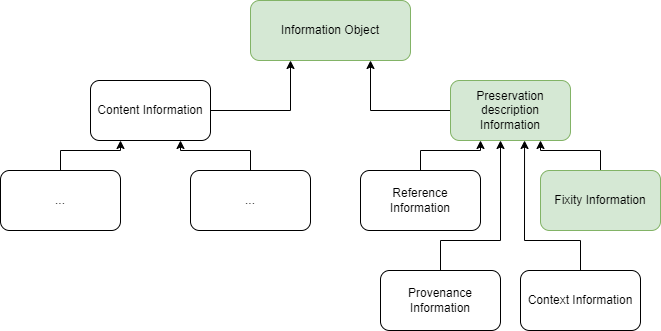
\includegraphics[width=0.7\textwidth]{oais.png}
  \caption{The transaction hash, used to retrieve data from the blockchain, is stored in the fixity information of the PDI of an information object \cite[7]{lee2010open}.}
  \label{fig:oais-fixity}
\end{figure}

The \textit{Artifact} is a combination of decentralized application on the Ethereum blockchain and a local pool structure in the archive. The smart contract exposes functions for managing cryptographic hashes of pools.
The artifact must provide the following functionalities:
\begin{itemize}
  \item Create, Read, Update SHA256 values of pools.
  \item Must hold a reference (ID) for the respective pool in the archive.
  \item Must be tamperproof for unauthorized calls.
\end{itemize}
The smart contract complements the local pool structure in the archive where fixity information of certain object pools may be requested on any given time. The artifact should reduce the amount of operations needed to ensure the integrity of 10,000 objects from ingest to retrieval process by at least 50\%.

\section{Structure of the work}
The remainder of this work is structured as follows:
\begin{enumerate}[label=\textbf{\arabic*})]
  \setcounter{enumi}{1}
  \item \textbf{Related Work} presents the state of the art of projects that utilize the Ethereum blockchain as a storage medium for metadata
  \item \textbf{Diplomatics of Digital Records} gives an overview of the abstract concept of trust in digital archives
  \item \textbf{Ethereum Blockchain} gives an overview of the concepts and functions of the Ethereum ecosystem
  \item \textbf{Fixity Storage} contains an introduction to fixity information and how to handle it, this chapter also contains the implementation and deployment of the fixity storage utilized in this work
  \item The \textbf{Evaluation} chapter contains the answers to the research questions 
  \item I interpret and explain the results in the \textbf{Discussion} chapter
  \item \textbf{Conclusion} suggests future work and my contribution to the digital preservation research field
\end{enumerate} \chapter{Related Work}
\section{Project Archangel}
Project ARCHANGEL is a decentralized fixity information developed in the UK with the participation of three other countries, Australia, Estonia and Norway. Their approach is to store a cryptographic hash of every incoming object of the archive on a proof-of-authority blockchain. The project started in 2017 and ended in August 2018. The goal of the project was to ensure the integrity and authenticity of digital objects in archives with the usage a private fork of the Ethereum network. Their design philosophy of operating a private blockchain has the flaw of giving a few entities the power to alter data on the blockchain. Currently, their implementation uses smart contracts as a gateway for writing to the Blockchain \cite[4]{collomosse2018archangel}.

The public's trust in Archives and Memory Institutions (AMIs) has eroded, according to the authors of the project ARCHANGEL, due to the ease with which forgery and unauthorized modifications to electronic records can be carried out due to advances in technology and the creation of numerous types of composited content. Unlike in the past, when archives relied on specific firms' products and technologies, blockchain introduces a whole new paradigm of openness and expandability. The blockchain grants permission to write records in a distributed ledger to only authorized institutions, whereas permission to view the recorded content is granted to every node participating in the blockchain. Furthermore, scalability permits the use of diverse open-source tools and the assurance of record integrity by several parties through a consensus mechanism rather than by a single centralized organization. \cite[4]{wang2021research}.
The proposed architecture of ARCHANGEL can be seen in Figure \ref{fig:archangel} where the cryptographic hash of an incoming object is computed and then persisted onto the private blockchain. After a certain time interval, the object can be retrieved from the archived and a hash will be recomputed with the same cryptographic hash function. The object is guaranteed to be unaltered if the local and online hash value are the same.
\begin{figure}[t]
    \centering
    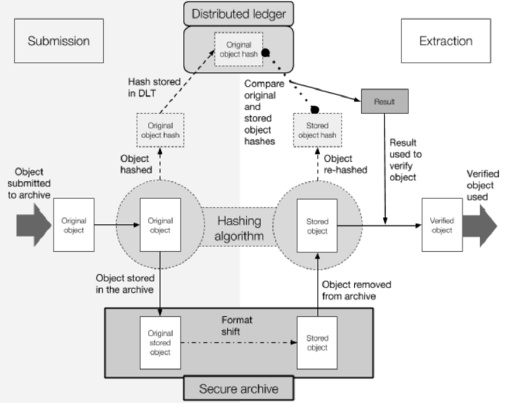
\includegraphics[width=0.5\textwidth]{archangel.png}
    \caption{Architecture of the ARCHANGEL platform \cite[2]{collomosse2018archangel}.}
    \label{fig:archangel}
\end{figure}
I agree with their vision of publicly available fixity information, where everyone with an Ethereum client is able to validate the integrity of objects in archive, but there are two points which do not conform with my vision. First and foremost is the usage of a private fork of the Ethereum network that is operated by a private set of nodes, which is basically a proof-of-authority consensus mechanism and contradicts the vision of a decentralized application \cite[3]{collomosse2018archangel}. Second, their implementation can hardly be used on the public Ethereum blockchain instead of a private fork due to the high cost of persisting data on the Ethereum main net, which is about \$8 for a SHA256 value, see Section \ref{sec:tx-cost}. 

\section{Provenance framework for the Internet of Things (IoT)}
Sigwart et al. (2020) proposed a data provenance framework for the IoT. Their approach is to store provenance records as so-called non-fungible assets on the Ethereum blockchain. Their prototype implements the ERC721 standard, which defines an interface for non-fungible assets or tokens (NFTs) which can be transferred by any clients (e.g., sensors, wallets), leaving a trail of provenance records created by passing the data NFT from owner to owner \cite[7]{Sigwart2020}. 
This project is important for my thesis, because it shows that the Ethereum blockchain can be utilized as a secure storage for immutable metadata which complements processes outside the blockchain.
Contrary to their implementation, I decided to not utilize the ERC721 standard since the data in my case, fixity information, does not need to be transferred from owner to owner. In order to use their implementation for fixity information instead of provenance data, you would have to deploy or "mint" an NFT for each digital object in the archive. That means, massive overhead in operation cost since "minting" is basically a deployment of a smart contract, which is one of the most expensive operations on the Ethereum blockchain, see Table \ref{table:gas-costs}.

\section{Pooled testing}\label{sec:pooled}
Pooled Testing was first introduced by \cite{dorfman1943detection} as a strategy to screen numerous military recruits for syphilis during World War 2. Dorfman envisioned that instead of testing each recruit's blood specimen separately, multiple specimens could be pooled together and tested at once. Positive pools' specimens would be retested individually to determine which recruits had contracted the disease, whereas negative pools' specimens would be declared negative. Dorfman wanted to save money on testing while still identifying all syphilitic-positive candidates, so he used group testing. Because the goal is to identify all positive persons among all individuals tested, this is now known as the "case identification problem." Dorfman's case identification method can be thought of as a two-stage hierarchical algorithm. Individuals from positive pools are tested in the second stage after non-overlapping pools have been screened in the first.

In this thesis, two strategies of pooled testing are implemented. 
First, two stage hierarchical pooling strategy, where in the first stage of this protocol N pools get initialized and filled with samples of the population. If the combined result of the pool is negative than no second stage is needed, but when a pool is declared positive a second stage is needed and all individuals from this pool have to be retested in order to find the corrupted individual. The expected number of test is equal to the number of tests in the first stage added to the number of tests in the second stage \cite[3]{nianogo2021optimal}.
Second, context-sensitive pooling, where homogeneous pool samples are grouped where it is assumed that the within-group change rate is smaller than the between-group change rate. Hence, if one member of a pooled group is corrupted, there is a high likelihood that other group members are also infected \cite[3]{deckert2020simulation}.

\section{Summary}
The blockchain related projects presented in this chapter have a common vision, which is a decentralized storage for metadata to validate the integrity and authenticity of data used in applications. The ability for the public to validate that an authority did not tamper with the data in their care is important and the removal of trust strengthens the trust in public institutions. More on the subject of trust can be seen in Chapter \ref{ch:diplomatics}
Decentralization and trust aside, the cost of the fixity storage presented in this thesis is also more than relevant as later seen in Chapter \ref{ch:ethereum}, where the cost and computational effort of interacting with the Ethereum network is presented.
 \chapter{Diplomatics of Digital Records}
\label{ch:diplomatics}
\section{About Diplomatics}
Diplomatics is a science founded in France in the seventeenth century by Benedictine monk Dom Jean Mabillon in his dissertation De Re Diplomatica Libri VI (1681) to determine the provenance and authenticity of evidence attesting to patrimonial rights. It was then utilized by attorneys to settle disputes, historians to interpret documents, and editors to publish medieval deeds and charters, and it evolved into a legal, historical, and philological specialty.
Classic diplomatics and modern/digital diplomatics should be distinguished since these two areas of the field do not represent a natural evolution of the latter from the former, but rather operate in parallel and focus on separate topics. Modern diplomatics encompasses all documents produced in the course of any kind of business, and is defined as "the discipline that studies the genesis, forms, and transmission" of records, as well as "their relationship with the facts represented in them and with their creator, in order to identify, evaluate, and communicate their true nature."

Both classic and modern diplomatics are concerned with determining the trustworthiness of records; however, the former does so retrospectively, examining records from several centuries ago, whereas the latter is concerned not only with establishing the trustworthiness of historical information but also with ensuring the trustworthiness of records yet to be created \cite[10]{kirschenbaum2010digital}. 

A digital record is a digital component, or group of digital components, that is saved, treated, and managed as a record, or, more specifically, a record whose content and form are encoded using discrete numeric values, such as the binary values 0 and 1, rather than a continuous spectrum of values, as defined by modern diplomatics. A digital record differs from analogue and electronic records in that it is digital. The representation of an item or physical process using continuously varying electronic signals or mechanical patterns is referred to as analogue by InterPARES\footnote{InterPARES 2, Terminology Database, \url{http://www.interpares.org/ip2/ip2_terminology_db.cfm} (accessed on 25 April 2022)}.
An analogue depiction of an object or physical process, in contrast to a digitally recorded representation, closely mimics the original. Any analogue or digital record conveyed by an electrical conductor and requiring the use of electronic equipment to be comprehensible by a person is defined as an electronic record by InterPARES. Using the classic archive idea, InterPARES defines a record as a document created or received as an instrument or by-product of a practical activity and set aside for action or reference \cite[44]{duranti2009digital}.

The integrity of a record is determined not only by its appearance – which can be deceiving in the case of good forgeries – but also by the circumstances of its maintenance and preservation: until proof to the contrary, an unbroken chain of responsible and legitimate custody is considered an insurance of integrity, and integrity metadata are required to attest to that. The duty for a record's authenticity changes from the creator's trusted record keeper, who must guarantee it for the duration of the record's custody, to the trusted custodian, who must guarantee it for the duration of the record's existence \cite[53]{duranti2009digital}. In this thesis the Ethereum network acts as a trusted custodian which guarantees that no one is able to tamper with the fixity information of digital records.

There are no originals in the diplomatic sense in the digital environment since there are no records that are the first instance of an item. When a digital record is closed for the first time, the original is destroyed and every time it opens a copy is created. However, it can be stated that each digital record is a copy in the latest version utilized by the creator, and that any version retained by the preserver is a genuine copy of the creators record.

\section{Trustworthiness}
Whether it is a stack of paper or a digital file, trustworthiness is a concept and an obligation that lasts the life of the document. As files go through the stages of the preservation process, from initial capture and metadata extraction to longer-term strategies like migration and rights management, the needs of born-digital objects change. Born-digital objects follow a similar path from creator to intermediary, such as a dealer or other (human or technology) agent, to archival repository staff, and eventually to storage and, possibly, ingest into a digital repository. The phases of that journey make up a digital objects chain of custody, and each one has a significant impact on the trustworthiness of the born-digital elements in a given accession.\newline The fundamental parts of creating and maintaining trust are the provenance of both analog and digital resources, as well as documentation concerning their storage environment, what has been done to them, and by whom. In the collection and preservation of born-digital resources, the trustworthiness of an institution, a custodian, or a document is critical \cite[27]{kirschenbaum2010digital}. 

Modern diplomatics concerns itself with four aspects of trustworthiness: reliability, authenticity, accuracy and authentication \cite[10]{kirschenbaum2010digital}.

\subsection{Reliability}
The content of a record's trustworthiness as a statement of fact. It is evaluated on the basis of 1) the completeness of the record, that is, the presence of all formal elements required by the legal-administrative system for that specific record to be capable of achieving the purposes for which it was created; and 2) the controls exercised on the process of creating the record, among which are those exercised on the author of the record, who must be the person competent, that is, having the authority and capacity to create the record.
The creator and trustworthy record keeper, that is, the person or organization who made or received the record and kept it with its other records, are solely responsible for its reliability \cite[52]{duranti2009digital}.

Archivist' expectations reliable sources have evolved over time, from the belief that librarians and archivists would provide researchers with verifiable evidence, to more modern understandings that reject the ideal of the reliable source and regard all texts as potentially deceptive and richly ambiguous. Data-stewards should be able to offer researchers with documentation about the provenance and acquisition of the data in their care using the methods of operation and processes created by the community and professionals, such as a provenance chain or the fixity information created on ingest of the object in question \cite[32]{kirschenbaum2010digital}.

Open source software is favorable in terms of reliability because community members can look into the code and verify that no unwanted actions will be executed. From a technical perspective, the blockchain suits as a source of reliability since it is well accepted by the public and every transaction ever made is publicly viewable and therefore fulfills the first point of reliability: completeness of the record. Also, the source code of the Ethereum network and each update (fork) gets peer reviewed and is available on GitHub\footnote{\url{https://github.com/ethereum/go-ethereum}}.


\subsection{Authenticity}
Authenticity refers to a record's ability to be trusted as a record, and is defined as the fact that a record has not been tampered with or corrupted, either accidentally or with malicious intend. An authentic record keeps the same identity it had when it was created and can be presumed or demonstrated to have kept its integrity across time. The identity of a record is made up of all the features that set it apart from other records, and it is determined by the formal components on the record's face and/or its attributes, as stated in a register entry or as metadata \cite[52]{duranti2009digital}.
With the fixity information stored on the blockchain, it can be proven that a record in the archive has not been tampered with. The simple comparison of the hash values generated in different points in time can prove the authenticity of a record.

\subsection{Accuracy}
Because record correctness was subsumed under both trustworthiness and authenticity as a notion, it was never a consideration in general diplomatics. Accuracy is defined as the truthfulness, exactness, or completeness of the data (i.e., the smallest, meaningful, indivisible pieces of information) within a record. Because of the ease with which data can be damaged during transmission over space (between humans and/or systems) and time in the digital environment, accuracy must be considered and assessed as a separate quality of a record (when digital systems are upgraded or records are migrated to a new system). As a result, the responsibility for accuracy shifts over time from the creator's trusted record-keeper to the trusted custodian \cite[52]{duranti2009digital}.
Whether it is a bit-rot or any other unintended error during the preservation process, a cryptographic hash value will be different if any bit of the object in the archive has changed and therefore the system presented in this thesis fulfills the requirements of accuracy.

\subsection{Authentication}
Authentication is defined as a statement or an element, such as a seal, a stamp, or a symbol, attached to a record after it has been completed by a competent employee. Authentication simply assures that a record is authentic at one precise point in time, when the declaration is made or the authenticating element or entity is affixed, whereas authenticity is a quality of the record that accompanies it for as long as it remains as is. A digital signature is frequently used in the digital environment to give ultimate authenticity. Because it is tied to a full record, the digital signature serves as a seal, allowing verification of the record's origin and integrity, as well as making the record unassailable and incontestable by performing a non-repudiation function. \cite[53]{duranti2009digital}.
Authentication in this process is not intended, since I do not use any form of digital signature to prove that a record is indeed authentic on ingest. In this thesis, I assume that every object is authentic and reviewed by a competent employee.

\section{Summary}
The concept of trust in a public authority is presented in this chapter and acts as a foundation for designing the fixity storage. The concept of authenticity is implemented through the usage of SHA256 values in this thesis, where the collision resistance of the SHA256 algorithm guarantees that no object in the archive can be tampered with. Accuracy is also guaranteed through the usage of a cryptographic hash function, since the hash is completely different if a bit level error happens over the course of the preservation.
Reliability is enforced by the nature of the blockchain, where every state changing action is documented immutable as long as the blockchain exists, as later presented in Chapter \ref{ch:ethereum}. Each of the core concepts of trust is needed in the modern digital world, where it is easier than ever to manipulate data and opinions. 
\chapter{Ethereum Blockchain}
\label{ch:ethereum}
\section{Introduction to Ethereum}
\label{sec:eth-blockchain}
Open source blockchain networks like Ethereum and Bitcoin are software kits that allow you to create an economic system in software, replete with account management and a native unit of exchange that can be used to transfer funds between accounts. These native units of exchange are referred to as coins, tokens, or cryptocurrencies, but they are the same as tokens in any other system: they are a type of money that can only be used within that system to pay peers or run programs on the Ethereum network.
When you want to make one of these peer-to-peer networks accessible through a web browser, you need to use special software libraries such as Python's Web3\footnote{\url{https://github.com/ethereum/web3.py}} which is utilized in this thesis to connect to the Ethereum network \cite[2]{dannen2017introducing}.

The fact that everyone in the world can interact with the blockchain, given you have internet access and an according device, such as a PC or mobile phone, is advantageous for a fixity storage such as presented in Chapter \ref{ch:fixity-storage}. Anyone is able to validate the integrity of an object with the right resources, e.g., the transaction in which an object's fixity information was originally stored. Picture a digital archive which releases multiple objects to the public and their respective fixity information on the blockchain, the community could then validate if the object in question is authentic. Pure trust, that an archive or its stewards did not tamper with the data in their care is therefore not needed anymore.
\section{About the Ethereum blockchain}
A block is a time unit that contains a specific amount of transactions. Transaction data is captured throughout that time period, and when the unit of time expires, the next block begins. The blockchain is a representation of the history of state changes in the Ethereum network \cite[43]{dannen2017introducing}.
The Ethereum network divides transactions and state changes into blocks, which are then hashed. Before the following canonical block may be added on top of it, each block is inspected and validated. Nodes on the network will no longer need to evaluate the trustworthiness of every single block in the Ethereum network's history, but only validate the most recent block in the chain. Therefore, it gets harder to tamper with past transactions with each block set on top of the blockchain. The blockchain is made up of all the blocks strung together, including the genesis block, which is the first block in the blockchain. The blockchain is also known as a distributed ledger or \acrlong{dlt} (\acrshort{dlt}). The term ledger is correct since the chain contains every transaction in the network's history, thereby turning it into a massive, well-balanced ledger \cite[55]{dannen2017introducing}. 
\section{Ethereum Virtual Machine (EVM)}
\label{sec:evm}
The physical manifestation of the \acrshort{evm} exist as a single entity sustained by thousands of connected computers running an Ethereum client\footnote{\url{https://ethereum.org/en/developers/docs/evm/}}.
In the Ethereum context, a virtual machine is a massive global computer made up of constituent nodes, which are themselves computers. In general, a virtual machine is a computer system that is emulated by another computer system. These emulations are based on the same computer architectures as the target of their emulation, but they usually reproduce that architecture on hardware other than that for which it was designed. Virtual machines can be built using hardware, software, or a combination of the two. It is both in the case of Ethereum. Rather than securing thousands of individual machines, Ethereum takes the approach of securing one massive state machine that can span the entire globe \cite[48]{dannen2017introducing}.

The \acrshort{evm} can run any computer program written in Solidity\footnote{\url{https://github.com/ethereum/solidity}}, the native programming language of the \acrshort{evm}. These programs will always create the same output, with the same underlying state changes, when given a specific input. As a result, Solidity programs are entirely deterministic and guaranteed to execute, as long as you pay enough for the transaction. Solidity programs are Turing complete in the sense that they can express all tasks that can be performed by computers. This means that every application executed on the platform is run by the entire dispersed network, every node \cite[50]{dannen2017introducing}.

The \acrshort{evm} is also a runtime environment for small programs that can be executed via a network, from the perspective of a software developer. Smart contracts are compiled into the \acrshort{evm}'s native language, the \acrshort{evm} bytecode. By using a client application like Truffle\footnote{\url{https://trufflesuite.com/}} or Geth\footnote{\url{https://geth.ethereum.org/}}, Solidity, a high-level language, is compiled into bytecode and posted onto the Ethereum network \cite[51]{dannen2017introducing}. I have decided to utilize Truffle for this thesis because of its fast and easy way to interact with the Ethereum network and its subnetworks.
\section{Smart Contracts}
Smart contracts, similar to the concept of classes in traditional object-oriented programming, are the building blocks of decentralized apps operating on the \acrshort{evm}. When developers talk about developing smart contracts, they usually mean writing applications in the Solidity programming language for execution on the Ethereum network \cite[10]{dannen2017introducing}.
In my thesis, the fixity storage is often referred to as \acrlong{dapp} (\acrshort{dapp}), which is an application built with several smart contracts. The smart contract implemented in this thesis is further described in Section \ref{sec:implementation}. 

\section{Persistence}\label{sec:persistence}
Decentralized storage systems, unlike centralized servers managed by a single corporation or organization, are made up of a peer-to-peer network of users that each hold a share or the full amount of the data, resulting in a resilient file storage sharing system. All transactions in Ethereum are stored on the blockchain, a canonical history of state changes stored on every single Ethereum node \cite[12]{dannen2017introducing}. 
The chain is steadily growing and on March 19, 2022, the Ethereum chain is at 602.95 GB\footnote{\url{https://ycharts.com/indicators/ethereum_chain_full_sync_data_size}}, which every node on the network needs to be able to store. If the chain were to expand to large amounts of data (say 5TBs) it would not be feasible for all nodes to continue to run. Also, the cost of deploying this much data to the mainnet would be prohibitively expensive due to fees\footnote{\url{https://ethereum.org/en/developers/docs/storage/}}.
My proposed solution utilizing is pooled testing in order to mitigate the ever-increasing chain size of the Ethereum network by reducing the amount of transactions needed to operate the fixity storage. 

The blockchain, as a decentralized storage system also follows some rules, constrain and enforce relationships between entities. Motives to break or alter these relationships can be found in a wide range of industries, leading to bribery and corruption and making blockchain's trustless properties even more appealing to businesses than previous generations of software and networking. Shared read/write access generates considerable complexity. Depending on where the client's machine is located and regarding its internet speed, machines all over the world may experience variable latency, resulting in certain write operations arriving out of order. This becomes even more challenging when numerous parties are expected to share the blockchain equally \cite[20]{dannen2017introducing}. The Ethereum network solves this problem by nodes executing any code included within a block independently, this is possible due to the deterministic characteristic of the Solidity programming language. This method is not only highly parallelized, but also very redundant. Despite the significant redundancy, this is a reliable and efficient technique to balance a worldwide ledger \cite[50]{dannen2017introducing}.

Ethereum requires a persistence mechanism in order for a piece of data to last indefinitely. When executing a node, for example, the persistence method requires that the entire chain be considered. The chain continues to grow as new pieces of data are added to the end, requiring each node to reproduce all the embedded data. The term for this is "blockchain-based persistence." The problem with blockchain-based persistence is that the chain could grow to be far too large to maintain and retain all the data in a reasonable amount of time (e.g., many sources estimate the Internet to require over 40 Zetabytes of storage capacity). 

In addition, the blockchain must have some sort of incentive system for the participating nodes in the network to validate new blocks in the blockchain. Validating a block is a computational hard task which requires nodes to have a vast computing power which is used in a consensus mechanism called proof-of-work. In this consensus mechanism a cryptographic puzzle has to be solved, by the node which aims to validate a block, in order for a block to be seen as valid. The node which solves the puzzle and therefore presents the proof-of-work is rewarded with the so-called block-reward in form of \acrlong{eth} tokens. Ether is the name of the token, or cryptocurrency which is mainly used in the Ethereum ecosystem to pay for transactions or to fuel smart contracts. Ether can be publicly traded into other currencies such as EUR or USD.

For blockchain-based persistence, the incentive system includes a payment made to the miner, the payment varies with the amount of data which has to be included in a block\footnote{\url{https://ethereum.org/en/developers/docs/storage/}}.

\section{Test Networks}\label{sec:test-nets}
There are multiple independent networks implementing the Ethereum protocols, since the Ethereum source code is openly available everyone is able to set up an Ethereum network, which is often called a private fork. Networks can also be utilized as different Ethereum environments for development, testing or production use cases. The private key for an Ethereum account works across various Ethereum networks, but the transaction history or account balance is independent for each network, meaning you can not transfer funds from a test network to the mainnet and vice-versa. For testing purposes, I have utilized the Ropsten test network to deploy and interact with the fixity storage presented in Section \ref{ch:fixity-storage}. Interactions on the test network also requires you to have some funds in your wallet to pay for transactions, although the funds on the test network does not require you to gather them from exchanges for money. The \acrlong{eth} token for the Ropsten test network can be acquired through public faucets, where you receive some tokens after you have input your wallet address. Some faucets require you to have a Twitter account (e.g., \url{https://faucet.paradigm.xyz/}), with a certain amount of tweets and follower for bot protection and some faucets do have a large waiting queue for Ether tokens, in the case of \url{https://faucet.dimensions.network/} the waiting time can reach up to three days. Faucet are usually time gated, meaning that you could request \acrlong{eth} tokens only once per day. At small scale, this limitation is no problem for this thesis because persisting around ten pools on the blockchains require at max 0.002 \acrlong{eth} tokens. The one per day paradigm gets problematic for the experiment including 10,000 objects, which costs about 20 \acrlong{eth} tokens, which means I would have to request tokens for 20 days straight to perform one experiment on a real live environment such as the Ropsten test network. I have utilized each before presented faucet to gather funds for the experiment, my suggestion for future work is to use the following Ropsten test network faucet: \url{https://faucet.egorfine.com/}. This faucet does require you to either have an active social media account, neither does it implement a waiting queue.
There are multiple options to choose from for a testnet, from the most prominent networks presented at the official Ethereum documentation\footnote{\url{https://ethereum.org/en/developers/docs/networks/}} only the Ropsten test network implements the proof-of-work algorithm, which means it is the best representation of Ethereum to date, and for that reason I decided to utilize the Ropsten test network in my thesis.

\section{Gas and Fees}
\label{sec:costs}
Gas refers to the unit that measures the amount of computational effort required to execute specific operations on the Ethereum network, this property allows you to calculate the operation cost for the fixity storage without taking the price fluctuation of ETH into account. Since each Ethereum transaction requires computational resources to execute, each transaction requires a fee.
Gas fees are paid in \acrlong{eth} tokens. Gas prices are denoted in \acrlong{gwei}, which itself is a denomination of \acrshort{eth} - each \acrshort{gwei} is equal to 0.000000001 ETH. For example, instead of saying that your gas costs 0.000000001 \acrlong{eth}, you can say your gas costs 1 \acrlong{gwei}. The word "\acrlong{gwei}" itself means "giga-wei", and it is equal to 1,000,000,000 wei. Wei itself is the smallest unit of the \acrlong{eth} token\footnote{\url{https://ethdocs.org/en/latest/ether.html}}.

Miners are paid in \acrlong{eth} tokens for validating blocks, and also for running scripts on the network. The cost associated with electricity consumption of nodes running the Ethereum network is one of the factors that gives \acrlong{eth}, as a cryptocommodity, its intrinsic value—that is, someone paid real money to their electricity company to run their mining machine. Specialized mining rigs, which use arrays of graphics cards to increase their odds of solving the cryptographic puzzle in the proof-of-work mechanism, and therefore completing a block and collect the block-reward \cite[12]{dannen2017introducing}. 
Mining creates the consensus needed to make legitimate state changes in the distributed ledger, and miners are compensated for their contributions. This is how \acrlong{eth} tokens and Bitcoins are created \cite[57]{dannen2017introducing}. 
To ensure that the system is not clogged by meaningless spam contracts, there must be a fee associated with each instruction the \acrshort{evm} executes. An internal counter maintains the amount of the fees incurred each time an instruction is executed, which are then charged to the user. When a user initiates a \gls{transaction}, a tiny percentage of the user's fund is set aside to pay these fees \cite[58]{dannen2017introducing}. 

The costs are the driving factor of my thesis where I try to make as few transactions as possible to run a fixity storage on the Ethereum network. 
The fees are determined by the transaction's gas cost; gas is a unit of effort, not a subcurrency, therefore it cannot be held or hoarded. In computer words, it simply assesses how much work each step of a transaction will take. You need enough \acrlong{eth} tokens in your account to be able to pay for the transaction, or else it will get reverted. There is no need to buy gas individually because there is no gas token. Gas prices ensure that network computing time is adequately priced and varies with the time of the day, meaning the more traffic there is on the network the higher are the gas prices for transactions or smart contract calls \cite[59]{dannen2017introducing}.
The only person who suffers if you transmit a set of computationally difficult commands to the \acrshort{evm} is you, it has no bearing on the transactions of others. There is no method to jam the \acrlong{evm} without spending a significant amount of money in transaction fees. The gas price system serves as a de facto means of scalability. Miners have complete control over which transactions they will include in a block, depending on which transaction pays the highest fee rates, as well as the block gas limit. The block gas limit sets the maximum amount of processing and storage that can be done per block \cite[60]{dannen2017introducing}. 

\section{Transactions}\label{sec:tx-cost}
An Ethereum transaction refers to an action initiated by an externally-owned account, in other words an account managed by a human, not a contract. For example, if Bob sends Alice 1 \acrshort{evm}, Bob's account must be debited and Alice's must be credited. This state-changing action takes place within a transaction. It is a mechanism for an external account to provide the \acrshort{evm} instructions to do a task. To put it another way, it is a method for an external account to send a message to the system. A transaction in the \acrshort{evm} is a cryptographically signed data package storing a message, which tells the \acrshort{evm} to transfer tokens, create a new smart contract, interact with an existing one, or perform some calculation. Contract addresses, like users with external accounts, can be transaction recipients \cite[60]{dannen2017introducing}. 
\begin{figure}[t]
    \centering
    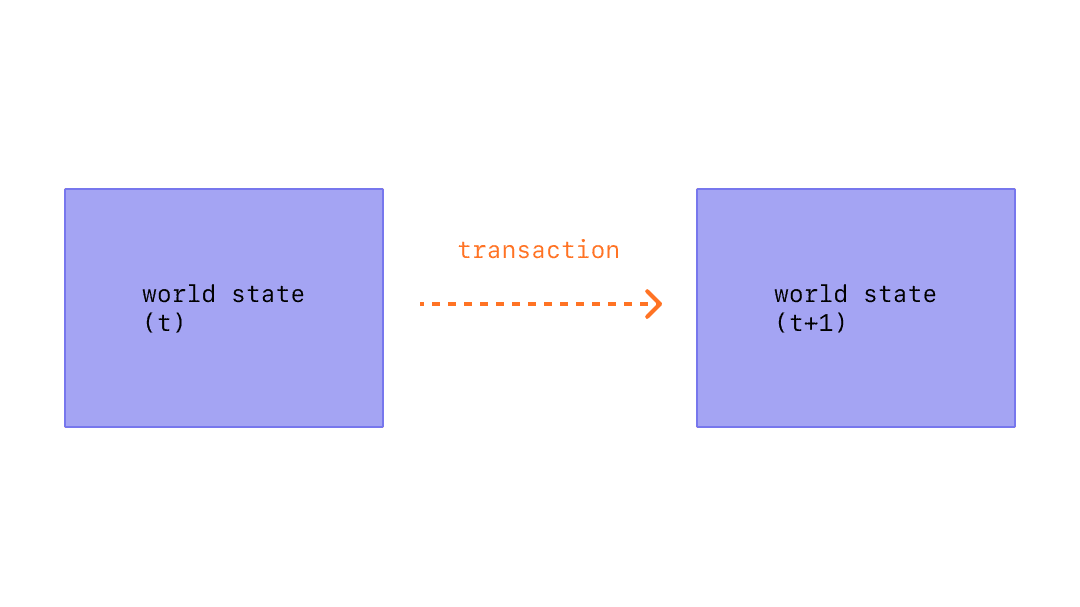
\includegraphics[width=0.5\textwidth]{eth_transaction.png}
    \caption{Illustration of an Ethereum transaction \url{https://ethereum.org/en/developers/docs/transactions/}}
\end{figure}
Transactions that affect the \acrshort{evm}s state must be broadcast to the entire network. A miner will execute the transaction and propagate the resulting state change to the rest of the network once any node broadcasts a request for a transaction to be conducted on the \acrshort{evm}\footnote{\url{https://ethereum.org/en/developers/docs/transactions/}}.
Transactions, which do not alter the global state are free of charged and are referred to as Calls. As seen in the source code in Listing \ref{lst:fixity-storage}, \textit{getPoolHash(uint32 poolId)} is marked with the keyword \textbf{view}, which means the function itself does not alter the state of the network. Contrary to the function \textit{setPoolHash(uin32 poolId, bytes32 poolHash)} which does alter the networks state and therefore generates cost for the fixity storage. In this thesis, writing actions on the blockchain are often referred to as Transactions; and reading actions are referred to as Calls.
Table \ref{table:gas-costs} presents the gas cost of the most relevant network operations used in this thesis according to the Ethereum yellow paper \cite[27]{wood2014ethereum}.
\begin{center}
    \begin{tabular}{ l l l }\label{table:gas-costs}
        Operation Name & Gas Cost & Description \\ 
        $codedeposit$ & 200 & gas cost per byte the compiled smart contract \\  
        $txcreate$ & 32000 & create a new smart contract  \\   
        $transaction$ & 21000 & base cost for a transaction \\
        $txdatazero$ & 4 & gas cost for every zero byte of the transaction data  \\   
        $txdatanonzero$ & 16 & gas cost for every non-zero byte of the transaction data  \\   
        $sset$ & 20000 & set a persistent variable for the first time in the contract \\
        $sreset$ & 2900 & the cost for updating a persistent variable 
    \end{tabular}
\end{center}

\section{Summary}
The learnings in this chapter is on how to interact with the Ethereum network, which tools to use and how the computational cost comes about. I have presented that it is important to prune all unnecessary transaction and storage data to mitigate the ever-increasing chain size of the Ethereum blockchain and reduce the cost for the user of the fixity storage presented in Chapter \ref{ch:fixity-storage}.  \chapter{Fixity Storage}
\label{ch:fixity-storage}
\section{Fixity Information}
Fixity Information provides the data integrity checks or validation/verification keys used to ensure that the particular Content Information object has not been altered in an undocumented manner\cite[8]{lee2010open}. In this thesis, fixity information will be a transaction hash, with which the fixity information can be retrieved from the Ethereum blockchain.
With fixity information you are able to answer questions regarding the authenticity and integrity of an object, which supports assertions about the authenticity and trustworthiness of digital objects \cite[3]{ndsa2017fixity}.
\newline \textit{Have you received the files you expected?} When fixity information is provided with objects upfront, it can be used to validate that you have received what was intended for the collection.
\newline \textit{Is the data corrupted or altered from what you expected?}  Once you have generated baseline fixity information for files or objects, comparing that information with future fixity check information will tell you if a file has changed or been corrupted.
\newline \textit{Can you prove you have the data/files you expected, and they are not corrupt or altered?} By providing fixity information alongside content, you enable your users to verify that what they have is identical to what you say it should be. 

Fixity is a key concept for the long-term preservation and management of digital material for many reasons. Previous scholarship on fixity has shown its vital importance in discovering changes to data and all that this error-checking can imply: authenticity and renderability of files, trustworthiness of institutions, and system monitoring/maintenance. Despite the centrality of fixity to the field of digital preservation, there is little prescriptive guidance on when and how to create fixity information, where to store it, and how often to check it. This absence is not without reason, however: the incredible variety of organizational structures, priorities, staffing levels, funding, resources, and size of collections held by institutions that do digital preservation make it difficult to establish a single set of one-size-fits-all best practices \cite[38]{ndsa2017fixity}.
\subsection{Generating Fixity Information on Ingest}
 It is important to check the fixity
of content transferred to you when you bring it under your stewardship. Whenever possible, it is ideal to encourage content providers or producers to submit fixity information along with content objects. You can only provide assurance about the fixity of content overtime once you have initial fixity values, thus it is imperative to document fixity information as soon as possible. If fixity information is not provided as part of the transfer, you should create fixity information once you have received the materials \cite[4]{ndsa2014fixity}.

\subsection{Fixity Checks}
Most fixity procedures involve a computational method that takes a digital file as input and outputs an alphanumeric value; this output value is used as a baseline comparison each time the fixity check is rerun \cite[5]{ndsa2017fixity}
In addition to checking fixity before and after transfer, collections of digital files and objects should be checked on a regular basis. There are a range of systems and approaches focused on checking the fixity values of all objects at regular intervals. This could be monthly, quarterly, or yearly for example. The more often you check, the more likely you are to detect and repair errors \cite[4]{ndsa2014fixity}.
The information must be put to use, in the form of scheduled audits of the objects against the fixity information. Additionally, replacement or repair processes must be in place. Ideally these will have been tested before being needed. All of this is critical for bit-level preservation, but ensuring fixity does not mean that the object is or will be understandable. Long term access is also contingent on ones ability to make sense of and use the contents of the file in the future \cite[2]{ndsa2014fixity}.
The rate of fixity checking is going to be dependent on how quickly you can run the checks, the complexity of your chosen fixity instrument, and how much of your resources (e.g., CPU, memory, bandwidth) can be used for this operation. This can become a choke point as the amount of digital content increases but the infrastructure to perform the checks stays the same. In a situation like this, the fixity checking activities can adversely affect other important functions like delivery of the content to users.
\subsection{Fixity Instruments}
\begin{table}[p]
    \centering
    \begin{tabular}{c|p{0.4\textwidth}|p{0.4\textwidth}}
      Fixity Instrument & Definition & Level of Effort and Return of Investment\\
      \hline
      Expected File Size & File size that differs from the expected can be an indicator of problems, for example by highlighting zero byte files & Low level of effort and low level detail. File size is auto-generated technical metadata that can be viewed in Windows Explorer or other common tools. \\  
      \hline
      Expected File Count & File count that differs from the expected can be an indicator that files are either added or dropped from the package. & Low level of effort and low level detail. File count is auto-generated technical metadata that can be viewed in Windows Explorer or other common tools.  \\
     \hline
     CRC & Error detection code, typically used during network transfers. & Low level of effort and moderate level of detail. CRC function values, which are variable but typically 32 or 64 bit, are relatively easy to implement and analyze.  \\
     \hline
     MD5 & Cryptographic hash function & Moderate level of effort and high level of detail. CPU and processing requirements to compute the hash values are low to moderate depending on the size of the file. The output size of this hash value is the lowest of the cryptographic hash values at 128 bits.  \\
     \hline
     SHA1 & Cryptographic hash function & Moderate level of effort, high level of detail, and added security assurance. Due to its higher 160-bit output hash value, SHA-1 requires more relative time to compute for a given number of processing cycles CPU and processing time than MD5.  \\
     \hline
     SHA256 & More secure cryptographic hash function & High level of effort, very high level of detail, and added security assurance. With an output hash value of 256 bits, SHA-256 requires more relative time to compute for a given number of processing cycles CPU and processing time than SHA-1. 
    \end{tabular}
    \caption{Various Fixity Instruments \cite[6]{ndsa2017fixity}.}
    \label{tb:fixity-instruments}
\end{table}
For a given fixity instrument, see Table \ref{tb:fixity-instruments}, the harder it is to find two objects that result in the same fixity information, the more “collision resistant” that instrument is. This is important mostly for preventing the concealment of intentional changes to objects. For example, expected file size and expected file count are extremely vulnerable to collision: it is very easy for someone to replace an object with one that matches in file size. It is also possible (although unlikely) for an unintentional change (such as corruption or human error) to result in an object with the same fixity information for instruments that have low collision resistance. Of the fixity instruments described above, the cryptographic hash functions (MD-5, SHA-1, and SHA-256) are the most collision resistant; SHA-256 is recommended for applications where security is important. However, performing fixity checking and replacing damaged objects is critical for any preservation system, and using any fixity instrument is much better than none at all. Note that as the level of security of the hash function increases, so do the time and resources needed to compute \cite[7]{ndsa2014fixity}.

\subsection{Storage Medium}
\label{sec:storage-medium}
There are various storages to store fixity information, each of them has some advantages and disadvantages in terms of convenience, security and throughput.
\newline \textit{In object metadata records:} In many cases, you will want to record some file or object fixity information wherever you store and manage the metadata records. These metadata records are actually stored as discrete files or in databases. This is particularly useful for maintaining originally submitted or generated fixity information as part of the long-term object metadata. 
\newline \textit{In databases and logs:} For checks you run at given intervals you may not want to be constantly adding to your object metadata records. In this case, it makes sense to keep fixity information apart from the object in databases and logs that you can return to when needed.
\newline \textit{Alongside content:} Its often ideal to have fixity information right alongside the content itself. That way, if you have problems with other layers in your system, or want to transfer some set of objects, you still have a record of previous fixity values alongside your content. For example, the BagIt specification includes a requirement for a hash value for the bagged content alongside the content. Similarly, some workflows involve creating *.md5 files, which are simply text files with the md5 hash, named identically to the file it refers to, but with an additional .md5 extension.
\newline \textit{In the files themselves:} When a checksum is for a portion of a file, it may make sense to store the information directly in the file. Note that this only makes sense when storing sub-file fixity information within a file. Adding fixity information for an entire file to the file itself changes the file and therefore changes its fixity value \cite[7]{ndsa2014fixity}.
\newline \textit{Ethereum Blockchain:} In this thesis I have chosen the blockchain to be the storage-medium for the fixity information. Its immutable state and availability in addition to its novel use-case in digital archives have influenced my decision.
\section{Example of a fixity storage}
A fixity storage must persist any kind of fixity information, in my thesis SHA256 values, for long term and guarantee that the persisted content is unaltered until retrieval of the content. I have chosen the Ethereum network as a medium for persisting file fixity information, see Section \ref{sec:storage-medium} for my reasoning. In Figure \ref{fig:lifecycle} the lifecycle of fixity information is presented, where at some point in time the information is ingested into the storage and after a certain time interval the information is fetched and compared to the retrieved SHA256 value from the digital object of the archive. If both cryptographic hashes match, the object is guaranteed to be unaltered. 
\begin{figure}[t]
  \centering
  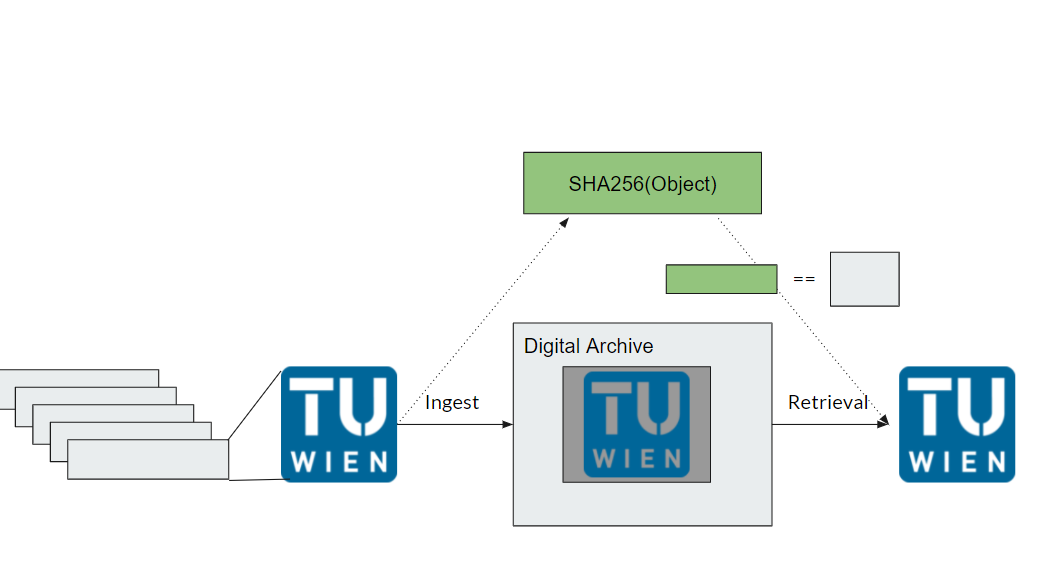
\includegraphics[width=0.75\textwidth]{lifecycle.png}
  \caption{Example of a fixity storage}
  \label{fig:lifecycle}
\end{figure}
\section{Implementation}
\label{sec:implementation}
The fixity storage presented in this thesis is implemented in Solidity, a programming language designed for the EVM, see Section \ref{sec:evm}.
The basic functionality of the smart contract, as described in Section \ref{sec:approach} can be seen in the source code presented in Listing \ref{lst:fixity-storage}
\begin{lstlisting}[language=Solidity,caption={MVP source code of the fixity storage deployed on the Ropsten test network \url{https://Ropsten.etherscan.io/address/0x0243c7aa552730E8C6F7ED25A480a7C0c88a70f0}},label=lst:fixity-storage]
// SPDX-License-Identifier: MIT
pragma solidity >=0.4.22 <0.9.0;

contract FixityStorage {
  mapping(uint32=>bytes32) pools;
  address creator;

  constructor()public{
    creator = msg.sender;
  }

  function getPoolHash(uint32 poolId) public view returns(bytes32) {
      return pools[poolId];
  }

  function setPoolHash(uint32 poolId, bytes32 poolHash) public {
    require(msg.sender==creator);
    pools[poolId]=poolHash;
  }
}
\end{lstlisting}
where \textit{getPoolHash(uint32 poolId)} implements a read function; \textit{setPoolHash(uint32 poolId,bytes32 poolHash)} implements create and update function. The mapping type is native in Solidity which implements a hash map consisting of a key and a value, where in this case the key is an integer representing the \textit{poolId} and the value is a \textit{bytes32} object representing the SHA256 root hash of the pool. The \textit{poolId} is the reference to the local pool in the digital archive, with which fixity information can be retrieved for a certain pool from the contract. The Solidity language presents a convenient  method to prevent unauthorized calls to the setPoolHash() method, which is \textit{require(msg.sender==creator)}. The native method \textit{require} is a "guard" function which improves the readability of the smart contract code and reverts the instruction if the condition is not met. The condition in this case is, that only the creator, which is set in the constructor, of the fixity storage is able to create and alter the information stored on the blockchain.

\section{Deployment}
I utilized truffle\footnote{\url{https://trufflesuite.com/index.html}} to run my deployment of the smart contract, it brings built-in smart contract compilation, linking, deployment and binary management with automated contract testing. The reasoning behind my decision is that, truffle has all the tools needed to implement a smart contract in one package and therefore reduced complexity in the development process. In the first iteration of the development process, I used the graphical user-interface Ganache\footnote{\url{https://trufflesuite.com/ganache/index.html}} to get a better feeling for the Ethereum blockchain, see Figure \ref{fig:ganache}.
\begin{figure}[t]
  \centering
  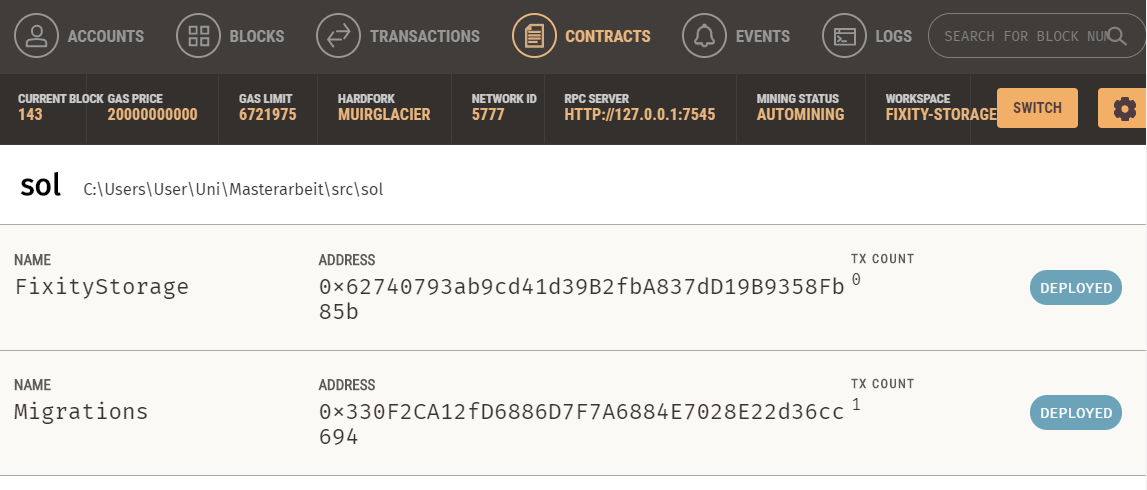
\includegraphics[width=0.7\textwidth]{ganache.png}
  \caption{Ganache, an interactive user interface for the Ethereum blockchain.}
  \label{fig:ganache}
\end{figure}
It allows you to navigate through your smart contract in a graphical user interface (GUI) and look at the state variables or functions to validate that your smart contract was successfully deployed. Ganache has a massive disadvantage when doing high throughput computing: it seems that it is not suited to withstand 10000 transactions built in a python for loop. Therefore, I only use the GUI it in the beginning of the experiment where I only persisted about 10 objects at a time without problems. For high throughput computing, truffle offers a command line tool to interact with the blockchain. The command line tool is resistant and shows no weakness when persisting 10,000 objects.
Truffle also allows to config other networks, e.g. the Ropsten test network, which can be defined as a parameter in the deployment process. The deployment requires to have some \acrlong{eth} tokens in your account to pay the miner to integrate your smart contract in a block. 
Truffle offers some utility regarding automated deployment, through the usage of deployment configurations where you can set the gas limit and the network configurations. Truffle offers a migrations feature, which is responsible for staging and versioning deployments. The migrations feature requires to have a smart contract deployed on the blockchain, which causes additional cost (191943 gas) to the fixity storage, therefore I have decided not to use the migrations feature, as it is controversial in the community and seen as unnecessary traffic and cost\footnote{\url{https://github.com/trufflesuite/truffle/issues/503}}.
The deployment cost of the smart contract can be calculated as follows:
\begin{equation}\label{eq:create-cost}
  \begin{split}
      C_{deployment} & = transaction + txcreate + codedeposit + txdatanonzero + txdatazero \\
      & = 21,000 + 32,000 + 200 \cdot 832 + 226 \cdot 4 + 800 \cdot 16 \\
      & = 233,104
  \end{split}
\end{equation}
where $transaction$ is the base cost for a transaction; $txcreate$ is the operation used to create a smart contract; $codedeposit$ is the gas cost for each byte of the runtime bytecode of the smart contract, which is 832 bytes and can be seen in the Input Data field of the transaction on \url{https://ropsten.etherscan.io/} with the following hash: \textit{0x844f76cfff6e00f29487f6fe3c99d8a69eab576e7c190e5b392745b48924a1f6}.
\textit{$G_{txdatanonzero}$} is 16 gas for each non-zero byte in the compiled bytecode of a transaction;\textit{$G_{txdatazero}$} is 4 gas for each non-zero byte in the compiled bytecode of a transaction; and \textit{$Contract_{bytesize}$} is the size of the compiled bytecode of the contract, see Section \ref{sec:costs} for the exact gas amount for each transaction.
The amount of gas consumed by the deployment of the decentralized fixity storage is 166,079 gas on the Ropsten testnet. The transaction used to deploy the contract can be found on \url{https://ropsten.etherscan.io/} with the following hash: \textit{0xf383c4bf0a5c32dd3369b02f68fd4e4400ef59343ad472bc96a28827f32c9abb}, where additional information, such as deployment date or the blocknumber, can be read. The address of the fixity storage, presented in Listing \ref{lst:fixity-storage} is \textit{0x0243c7aa552730E8C6F7ED25A480a7C0c88a70f0}.
\section{Authorized Access}
In Solidity one can require a certain address to access a function, the keyword \textit{requires} can be used so that a transaction from an unknown address can be reverted and only the owner of the creator address can update the mapped SHA256 values in the smart contract. An interesting topic is also how the private key in the archive may be managed, which is not part of this thesis, my suggestion for future work is a  multisignature wallet which can be used to split the responsibility of the contract owning Ethereum account, the creator account. Since the entity which controls the private key of the creator account is able to create and update fixity information on the blockchain. In the case of a compromised creator account, each entry of fixity information may be invalidated by the archive and new fixity information have to be uploaded to the blockchain. The key user management of the creators address may be investigated in further research. For this thesis I assume that the private key of the creator account is well managed and each transaction coming from the creator's address is legit.
\section{Cost of interacting with the fixity storage}\label{sec:cost-interating}
The cost of interacting with the fixity storage depends on the desired action. There are three different ways to interact with the contract: (1) create a new entry (2) update an existing entry and (3) read an entry.
The cost of a transaction, which invokes the \textit{setPoolHash} function and ultimately stores 256 bit on the blockchain can be calculated with Equation \ref{eq:tx-cost}
\begin{equation}\label{eq:tx-cost}
    \begin{split}
        C_{setPoolHash} & = gasAmount \cdot gasPrice \cdot ethPrice \\ 
        & = 42,368 \cdot 0.00000005 \cdot 4,000
    \end{split}
\end{equation}
which results in \$8.47 on average for an ETH price of \$4000.
The $gasAmount$ in Equation \ref{eq:tx-cost} can be calculated as follows:
\begin{equation}\label{eq:tx-data}
  \begin{split}
    gasAmount & = transaction + sset + txdatazero + txdatanonzero \\
     & = 21,000 + 20,000 + 16 \cdot 68 + 4 \cdot 70  \\
     & = 42,368
  \end{split}
\end{equation}
where $txdatazero$ is the number of zeros in the transaction data and $txdatanonzero$ is the amount of non-zero bytes in the transaction data. The transaction data for Equation \ref{eq:tx-data} can be found in the \textit{Input Data} field of the transaction on Etherscan\footnote{\url{https://ropsten.etherscan.io/tx/0x8839e03f0143bad34060fa909c35d30f2edb22dd4fdac0264de8ae84176eb1ea}}. This field contains the binary data that formed the input to the transaction, the structure is depending on which type of transaction is executed. Whether the transaction is contract call, contract deployment or message call the input data holds instructions in form of bytecodes to properly execute the desired interaction. The hexadecimal form of the input data is used for the calculation of $txdatazero$ and $txdatanonzero$.

The cost for updating an existing entry can be calculated in the same way as for creating ones, with the difference that the costly $sset$ operation can be spared and therefore updates costs 20,000 gas less than creates.
Reading an entry is free of charge, since no state changes has to be forwarded to the blockchain.
To explain the cost of the non-zero and zero bytes can be explained by looking the following \textit{Input Data} as a hexadecimal value:

\hash{0x178d292900000000000000000000000000000000000000000000000000000000000000001760d27083f6e2d1c46a65938c03a0c52dccf55cb4eb68a720e6efe3a8851f78}

where zero and nonzero bytes are counted and multiplied by their respective gas cost, which in this example is $txdatazero+txdatanonzero = 4 \cdot 70 + 16 \cdot 68 = 1368 $. The amount of non-zero bytes can be interpreted as the amount of effort given to the network.

\section{Proof of Concept}\label{sec:poc}
The proof of concept is written in Python in form of a Jupyter Notebook. It can be found on GitHub\footnote{\url{https://github.com/metsch/masterthesis/blob/main/src/py/poc_ropsten.ipynb}}. With Python's Web3.py I get the contract from the blockchain and extract its functions \textit{setPoolHash} and \textit{getPoolHash}. For the live experiment on the Ropsten test network I have initialized 100 digital objects, in form of SHA256 values, with a change rate of 0.1, meaning that \%10 of the ingested objects will be changed during the storage in the archive. The low amount of objects in the live experiment is due to the fact, that the Ropsten \acrlong{eth} token is hard to get, since the most relevant publicly available faucets are drained out and the ones available have a rate of only 0.1 \acrlong{eth} per day, as I explained in Section \ref{sec:test-nets}. I compute the optimal pool size k for N=100 and p=0.1 with Equation \ref{eq:poolsize} and created $\lceil N/k \rceil$ pools. Each pool is assigned a unique identifier and holds an array of objects, from which a hash list is formed, and the resulting root hash is later persisted on the blockchain. 
Before persisting the root hashes, I estimate the gas cost for a single transaction in order to set the gas limit, a transaction will revert if the cost exceeds the manually set gas limit. I utilized Equation \ref{eq:tx-data} and added 20\% in order guarantee that the transaction is not underpaid, which may happen if the network is congested at the time of firing the transaction.
At the time of the experiment, the gas price was 86.11 gwei which is 0,0000000896\acrshort{eth}, resulting in \$15.18 for a \textit{setPoolHash} transaction calculated with Equation \ref{eq:tx-cost} with an \acrshort{eth} price of \$4000. Admitted, this gas price is really high, usually the gas price is about 40 gwei. 
For each pool, 25 in total, I uploaded each root hash on to the blockchain and waited for the transaction to finish and run some tests to see if the transactions were successful.
After uploading the root hashes, I artificially corrupted the objects in the archive with a Bernoulli trial where an object gets corrupted if a random number between 0 and 1 is below p=0.1. At last, I repaired the archive by checking the local pools with the ones on the blockchain, and if the pool hashes did match the pool is seen as uncorrupted. Where the pools with non-matching hashes got replaced by copies of the objects.
To sum it up, the cost for the live experiment was for 25 writing transactions 0.11204969029 ETH (\$448) and 8 data-scrubbing operations resulting in 33 total operations. Data-scrubbing is an operation, where a corrupted object in the archive gets replaced with a fresh copy. The copy is assumed to be uncorrupted with the original hash value, therefore no further writing transaction is needed when you replace an object in the archive. Whereas, with an individual testing strategy the amount of writing transactions would have been 100 and estimated 10 data-scrubbing operations.

\section{Summary}
In this chapter I have presented the various forms of fixity information with their respective advantages and disadvantages together with my reasoning on why I have decided to utilize SHA256 cryptographic hashes. I have also presented various storage-media for fixity information and why it is so important that these storages guarantee for immutability in regard to history forgery. The interactions with the fixity storage are tested in an experimental environment, presented in the preceding section \ref{sec:poc}. \chapter{Evaluation}
\label{ch:evaluation}
The proposed fixity storage is evaluated on a local installation of the Ethereum blockchain and on the online Ropsten test network, where \acrshort{eth} tokens used for transactions are free of charge. The dataset used for evaluation is the format-corpus\footnote{\url{https://github.com/openpreserve/format-corpus}} from Open Preserve Foundation\footnote{\url{ http://openpreservation.org/}} on commit \textit{4e4b9a34540f72612ba6eab2d28bccceb7a848ae}\footnote{\url{https://github.com/openpreserve/format-corpus/commit/4e4b9a34540f72612ba6eab2d28bccceb7a848ae}} on the 16th of February.

I analyzed it to get a better understanding of various file formats, mostly on how volatile they are. The format-corpus is well-structured in a public GitHub repo with a decent amount of reputation in form of GitHub stars, where other datasets did provide corrupt links;were not available or did expect a lot of work to download them because they only allow single file downloads instead of bulks. Convenience; diversity of file extensions; and reputation of the organization affected my decision to use the format-corpus for analysis.
For the analysis I used the python package folderstats\footnote{\url{https://pypi.org/project/folderstats/}} which transforms a directory into a pandas\footnote{\url{https://pandas.pydata.org/}} dataframe. The repository contains 1560 files with 90 distinct file extensions, e.g. 986 \textit{.xml} files which are mostly PRONOM\footnote{\url{https://www.nationalarchives.gov.uk/PRONOM/}} registry files or \textit{pom.xml} files in case of java projects. 

In Figure \ref{fig:extension_distribution} you can see the distribution of file extensions where \textit{.xml} files make 62.2 percent of the portion and PDF with 6.79 percent as the second-largest portion.
\begin{figure}[t]
    \centering
    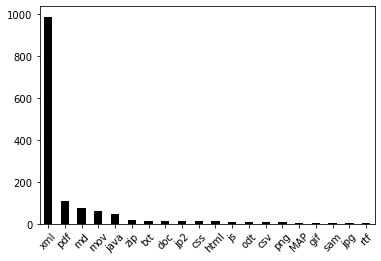
\includegraphics[width=0.5\textwidth]{extension_distribution.png}
    \caption{Distribution of file extensions in the format-corpus of Open Preserve Foundation. \url{https://github.com/openpreserve/format-corpus}}
    \label{fig:extension_distribution}
\end{figure}
To get a baseline estimate on how volatile certain extensions are due to updates and changes, I analyzed Git logs and count how many times a file extension was involved in a commit. The resulting column \textit{positives} was always higher or equal than the occurrence of a file extension, since each file was involved in at least one commit, the initial commit of the file. To count the commits I used the python package gitphyton\footnote{\url{https://gitpython.readthedocs.io/en/stable/}} and utilized the git command --log. For each file in the repository, I fired up the command \textit{git log --oneline filename} in python which resulted in one or multiple lines of logs. Later I used the multiline log as an input for the \textit{.splitlines()} function which results in an array of log lines, the length of this array minus 1 (the initial commit) is used to determine the new column \textit{positives} in the dataframe which shows if and how often a certain file has changed over the lifetime of the git repository. 
This method of determining the volatility of a certain file extension is by no means ideal, but there is no other method to check how often a certain file has changed without monitoring them on a system for a certain time interval. Therefore, I have decided to use the amount of file changes in the git repository as a rough estimate.
The change rate $p$ of a file extension is calculated with $positives/N$.

The two key parameters for evaluation are the operation cost and efficiency. 
\textit{Operation cost} \acrshort{op-cost} is calculated by multiplying the number of relevant cost transactions with the average gas cost for a \textit{setPoolHash} transaction on the blockchain, see Equation \ref{eq:expected_cost}
\begin{equation}\label{eq:expected_cost}
    \acrshort{op-cost} = \acrshort{count_wr} \cdot gasAmount
\end{equation}
where \acrshort{count_wr} is the number of write transactions on the blockchain; $gasAmount$ the amount of gas used for a writing operation, see Equation \ref{eq:tx-data}.
I intend to present the operation cost in the form of gas, the unit that measures the amount of computation effort required to execute specific operations, instead of the cost in USD or EUR. This is because, the amount of gas used during the experiment stays constant, whereas the price of the ETH token fluctuates heavily. Therefore, the amount of gas is a better indicator on how costly the fixity storage is.
\textit{Efficiency} \acrshort{eff} is measured by the number operations needed utilizing pooled testing compared O(\acrshort{two-stage}) with the individual testing strategy O(\acrshort{individual}), where the efficiency of pooling strategy S is expressed by Equation \ref{eq:efficiency}
\begin{equation}\label{eq:efficiency}
    \acrshort{eff} = O(S_{i})/\acrshort{count_op}
\end{equation}
where, assuming the preservation process of 10,000 digital objects without pooling requires O(\acrshort{two-stage}) operations and the preservation of the same objects using strategy S requires \acrshort{count_op} operations. In the case of individual testing the efficiency is 1, whereas if strategy S requires two times fewer operations the efficiency \acrshort{eff} is 2 \cite[4]{vzilinskas2021pooled}.

\textit{What is the optimal pool size based on the change rates of digital objects in the archive regarding cost and efficiency?}

Change rate $p$ represents the chance that an object will be changed , e.g., when I assume that 2,000 of 10000 objects will be changed or corrupted during the preservation process, $p = 2,000/10,000 = 0.2$. 

\textit{Operation Cost:} The optimal pool size, which will result in the lowest number of cost relevant transactions is the number of pools $J$, as seen in Equation \ref{eq:expected_writes}, because I only must write onto the blockchain during the ingest process where the root hashes of pools are persisted.
\begin{equation}\label{eq:expected_writes}
    \acrshort{count_wr} = J = \lceil N/k \rceil
\end{equation}
After the first iteration of the experiment, the number of corrupt objects per positive pools were included in the first draft of Equation \ref{eq:expected_cost}, where I assumed that I had to re-calculate corrupt pool hashes and re-store them on the blockchain, but these "repairing" actions can be done locally through data scrubbing. I only need to know that the pool is corrupt to substitute each object in the pool with a correct copy in the archive. For this part of the research question, local operations are out of scope because they do not cause direct cost on the blockchain, therefore the optimal pool size calculated by Equation \ref{eq:expected_cost} is $N$, see Figure \ref{fig:expected_cost}. A pool size of $N$ results in exactly 1 cost relevant transaction since I have combined every object on ingest into a hash-list which's root will be stored on the blockchain. This solution does not scale well, e.g., picture the process of retrieving a single object from the archive. In order to guarantee that the object is unaltered, I would have to re-compute the hash list from every object in the archive (or the bulk ingest in question). Additionally, if the single pool is corrupted, I must replace the whole bulk with copies. 
So, there must be an answer, which rewards smaller pool sizes to avoid too much data scrubbing. The number of data scrubbing operations is the number of objects in positive pools on retrieval and is calculated with Equation \ref{eq:expected_data-scrubbing},
\begin{equation}\label{eq:expected_data-scrubbing}
    R(S) = J_+ \cdot k = ((1-(1-p)^k)\cdot \lceil N/k \rceil) \cdot k
\end{equation}
where $(1-p)^k$ is the probability of a pool of size k being unchanged at a change rate of $p$ and the probability of a pool being changed is $1-(1-p)^k$. To find the optimal pool size regarding the amount of data scrubbing operations, I had to minimize Equation \ref{eq:expected_data-scrubbing}, as seen in Figure \ref{fig:expected_scrubbing}.
To find the optimal pool size in terms of operation cost and efficiency, operation cost and data scrubbing has to be accounted, which results in the final Equation \ref{eq:expected_operations}
\begin{equation}\label{eq:expected_operations}
    \acrshort{count_op} = J + J_+ \cdot k = \lceil N/k \rceil + ((1-(1-p)^k)\cdot \lceil N/k \rceil) \cdot k
\end{equation}
where \textit{J} is the number of pools and \textit{$J_+ \cdot k$} is the number of objects in corrupted pools. Therefore, the number of expected operations is the number of writing operations on ingest plus the number of data scrubbing operations on retrieval. By adding the amount of data scrubbing operations, the optimal pool size gets significantly lower, see Figure \ref{fig:expected_operations}. The optimal pool size \text{k} can be determined by finding the global minimum of Equation \ref{eq:expected_operations}, which results in the highest efficiency in Equation \ref{eq:efficiency}.
In the experiment, I have utilized Equation \ref{eq:poolsize} presented by \cite[3]{regen2020simple}, because it is more efficient than looking for the global minimum by force, and round the pool size up in order to avoid non integer pool sizes.
\begin{equation}\label{eq:poolsize}
    k = \lceil 1.24\cdot p^-0.466 \rceil
\end{equation}
\begin{figure}[t]\centering
    \begin{subfigure}{6cm}
        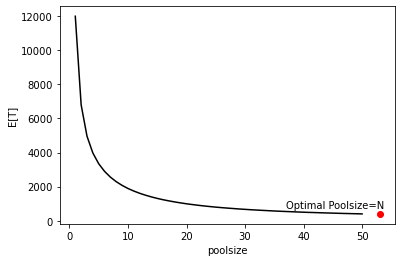
\includegraphics[width=\linewidth]{graphics/expected_cost.png}
        \caption{Optimal pool size regarding the writing transactions \acrshort{count_wr}.}\label{fig:expected_cost}
    \end{subfigure}
    \qquad
    \begin{subfigure}{6cm}
        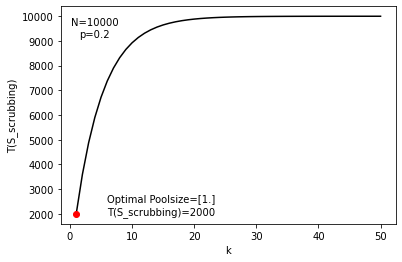
\includegraphics[width=\linewidth]{graphics/expected_scrubbing.png}
        \caption{Optimal pool size regarding the data scrubbing operations \acrshort{count_re}.}\label{fig:expected_scrubbing}
    \end{subfigure}
    \qquad
    \begin{subfigure}{6cm}
        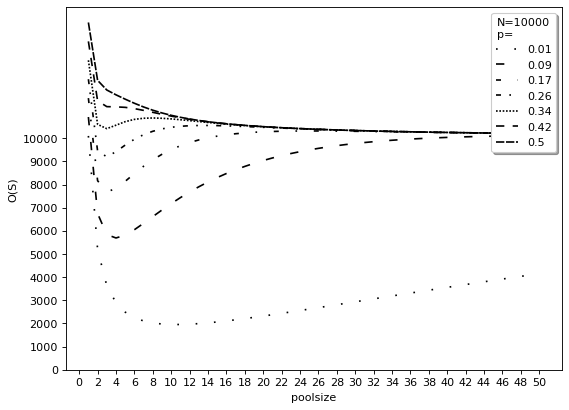
\includegraphics[width=\linewidth]{graphics/expected_operations.png}
        \caption{Optimal pool size regarding the total operations \acrshort{count_op} = \acrshort{count_re} + \acrshort{count_wr}.}\label{fig:expected_operations}
    \end{subfigure}
    \caption{Comparison of optimal pool sizes.}
\end{figure}
In Table \ref{tb:expected costs} and Figure \ref{fig:poolsizes} it is shown that for ingest bulks with higher change rates smaller pool sizes are favorable\footnote{\url{https://github.com/metsch/masterthesis/blob/main/src/py/rq1.ipynb}}.
The highest efficiency \acrshort{eff} can be achieved when the change rate is the lowest, where larger pool sizes are favorable, see Figure \ref{fig:poolsizes}.
\begin{figure}[t]\centering
    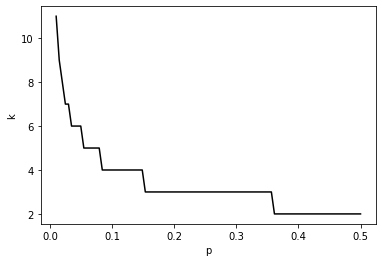
\includegraphics[width=0.5\textwidth]{graphics/poolsizes.png}
    \caption{Optimal pool sizes $k$ with change rate $p$.}
    \label{fig:poolsizes}
\end{figure}
\begin{table}[t]
    \centering
    \begin{tabular}{ c c c c c}
        N & p & k & E(\acrshort{two-stage}) & C(\acrshort{two-stage}) \\
        10000 & 0.010 & 11 & 5.16 & 11 \\ 
        \hline
        10000 & 0.05 & 5 & 2.39 & 5 \\  
        \hline
        10000 & 0.09 & 4 & 1.87 & 4 \\  
        \hline
        10000 & 0.14 & 4 & 1.62 & 4 \\  
        \hline
        10000 & 0.18 & 3 & 1.50 & 4  \\
        \hline
        10000 & 0.22 & 3 & 1.40 & 3  \\
        \hline
        10000 & 0.27 & 3 & 1.34 & 3  \\
        \hline
        10000 & 0.31 & 3 & 1.30 & 3  \\
        \hline
        10000 & 0.35 & 3 & 1.27 & 3  \\
        \hline
        10000 & 0.400 & 2 & 1.22 & 2  
    \end{tabular}
    \caption{Efficiency \acrshort{eff} and Cost Efficiency \acrshort{cost} of two-stage-hierarchical pooling compared to individual testing.}
    \label{tb:expected costs}
\end{table}

\textit{To what extent can pooled testing increase the efficiency and reduce cost for a fixity information storage service on the Ethereum blockchain?}

A context-sensitive approach in the medical field was proposed in 2020 were members of homogeneous groups were pooled, e.g. families, office colleagues or neighbors, and is proven to be more effective than individual testing \cite[4]{deckert2020simulation}. In this thesis, the idea of grouping similar files to increase efficiency of the pooling strategy, estimating their change rate and calculating the in-group efficiency as presented in Equation \ref{eq:efficiency}.
\begin{figure}[t]\centering
    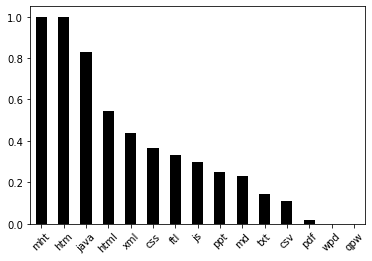
\includegraphics[width=0.5\textwidth]{graphics/p-distribution.png}
    \caption{Distribution of change rates $p$.}\label{fig:p-distribution}
\end{figure}
In Figure \ref{fig:p-distribution}, it is shown that the volatility in the repository only affects a few file extensions, where 77 out of 90 file extension where never altered and have therefore a $p$ value of 0.00. These unaltered file extensions are grouped with a group size of $Group_N$, which results in large bulks in the ingest process that have no impact on the retrieval since I assume that no object in this particular group will be altered during the preservation process. For instance, in Table \ref{tb:efficiency}, the file extension MOV has a change rate of 0.00 since no MOV was involved in a git commit. A change rate of 0.00 is not realistic, since a bit level error always may happen.
\begin{table}[t]
    \centering
    \begin{tabular}{ c c c c c c}
        extension & N & p & k & E(\acrshort{two-stage}) & W(\acrshort{two-stage}) \\
        \hline
        XML & 986 & 0.43 & 2 & 1.21  & 2.00 \\  
        \hline
        PDF &106 &0.01 & 8 &  3.60 & 7.57 \\
        \hline
        MD & 74 & 0.22  & 3 & 1.37 & 2.96 \\    
        \hline
        MOV&61 & 0.00 &  61 & 61.00 & 61.00 \\  
     \hline
     JAVA &47 &0.82 & 2  & 1.21 & 1.95 \\  
     \hline
     None & 26 & 0.00 & 26.0 & 26.00 & 26.00	 \\
     \hline
     ZIP & 17 &0.00 &  17 & 17.00 & 17.00 \\
     \hline
     TXT & 14 & 0.14 &  4 & 1.33 & 3.50 \\ 
     \hline
     DOC & 13 & 0.00 &  13 & 13.00 & 13.00 \\   
     \hline
     JP2 & 12 & 0.00 &  12 & 12.00 & 12.00 \\   
     \hline
     CSS & 11 & 0.36 & 2  & 1.07 & 1.83 \\  
     \hline
     HTML & 11 & 0.54 &  2 & 1.06 & 1.83
     \\   
     \hline
     JS & 10 & 0.3 & 3& 1.08 & 2.50
    \end{tabular}
    \caption{In group efficiencies of various file extensions.}
    \label{tb:efficiency}
\end{table}

To calculate the efficiency of the two-stage-hierarchical strategy, I have to sum up every changed file in the dataset which results in 510 changed files in the dataset. The change rate of the dataset is $510/1560$, which results in $0.32$. The input for Equation \ref{eq:expected_operations} is therefore N=1560; p=0.32 and k=3.0.
With context-sensitive pooling, another increase in efficiency can be made. In Table \ref{tb:context-sensitive} I compare the two strategies presented before, with respect to Equation \ref{eq:efficiency}, where the Two-Stage-hierarchical pooling algorithm has achieved an efficiency rate of 1.28 and context-sensitive pooling 1.38\footnote{\url{https://github.com/metsch/masterthesis/blob/main/src/py/rq2.ipynb}}. 
\begin{table}[t]
    \centering
    \begin{tabular}{c c c}
        Strategy & \acrshort{eff} & \acrshort{cost-eff} \\
        Individual & 1.00 & 1.00 \\
        Two stage hierarchical &  1.28 & 3.0\\
        Context Sensitive & 1.38 & 2.35
    \end{tabular}
    \caption{Efficiency of context-sensitive pooling vs. two stage hierarchical pooling.}
    \label{tb:context-sensitive}
\end{table}

\textit{Given that metadata has a higher change rate, what effect has the split of metadata and objects on the operation cost?}
To know what effect the split off metadata has, I had to double the initial 1560 file extensions and assign the postfix .meta to the newly created rows resulting in Table \ref{tb:metadata},
\begin{table}[t]
    \centering
    \begin{tabular}{c c}
        Extension & N \\
        METADATA & 1560 \\
        XML& 986 \\
        PDF& 106  \\
        MD& 74  \\
        MOV& 47  
    \end{tabular}
    \caption{Arbitrary set change rates $p$ in the format-corpus dataset.}
    \label{tb:metadata}
\end{table}
I calculate the efficiency for context-sensitive and two-stage hierarchical for various combinations of $p$ and $p_{meta}$ and the result is resulting in Table \ref{tb:split-off}. The combinations for $p$ and $p_{meta}$ are set arbitrary, future work may include the estimation of change rates based on the file sizes.
The Context-sensitive strategy never even reaches a 1.00 efficiency, which would state that it performs worse as the individual testing in terms of efficiency, this is due to the implementation of the context-sensitive strategy where the pool sizes cannot exceed the group size cannot exceed and loose the advantage of low change rates. In the two-stage-hierarchical I can group the metadata independently of the objects, resulting in 1560 objects with high change rate and 1560 objects with very low change rate. Although the performance is better than individual testing in terms of cost, the split off-metadata does have a worse effect on the overall performance due to the double amount of objects that have to be preserved\footnote{\url{https://github.com/metsch/masterthesis/blob/main/src/py/rq3.ipynb}}.
\begin{table}[t]
    \centering
    \begin{tabular}{c c c c c c}
        $p$ & $p_{meta}$ & E(\acrshort{cs}) & C(\acrshort{cs}) & E(\acrshort{two-stage}) & C(\acrshort{two-stage})\\
        0.001 &	0.99 & 0.77 & 1.71 & 0.86 & 1.91 \\
        0.007 &	0.96 & 0.73 & 1.60 & 0.80 & 1.76 \\
        0.013 &	0.94 & 0.71 & 1.55 & 0.78 & 1.69 \\
        0.019 &	0.91 & 0.69 & 1.49 & 0.76 & 1.62 \\
        0.026 &	0.89 & 0.68 & 1.46 & 0.74 & 1.58 \\
        0.032 &	0.86 & 0.67 & 1.46 & 0.73 & 1.58 \\
        0.038 &	0.84 & 0.67 & 1.42 & 0.72 & 1.52 \\
        0.044 &	0.81 & 0.66 & 1.42 & 0.71 & 1.52 
    \end{tabular}
    \caption{Various change rates $p$ and $p_{meta}$ in the format-corpus dataset compared with the individual testing strategy \acrshort{two-stage} where 1560 cost relevant transactions and 2070 operations are needed.}
    \label{tb:split-off}
\end{table}

The goal of this thesis was to reduce the cost of the fixity storage by at least 50\%, this goal can be met when the optimal pool size is at least two, which is guaranteed with a prevalence lower than 35.9\%, as seen in Figure \ref{fig:threshhold}.
\begin{figure}[tb]
    \caption{For a prevalence of corruption of maximum 35.9\%, an optimal pool size of at least two is guaranteed.}
    \label{fig:threshhold}
    \centering
    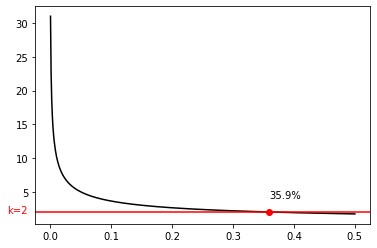
\includegraphics[width=0.5\textwidth]{threshhold.png}
\end{figure}
What happens if the prevalence is higher than 35.9\%, the optimal pool size would be between 1.0 and 2.0 which is not practical since a pool can not include 1.42 objects, therefore I have decided to round the result up from Equation \ref{eq:poolsize} which results in Figure \ref{fig:threshhold-ceil}.
\begin{figure}[tb]
    \caption{Round the resulting optimal pool size up to avoid non-integer pool sizes.}
    \label{fig:threshhold-ceil}
    \centering
    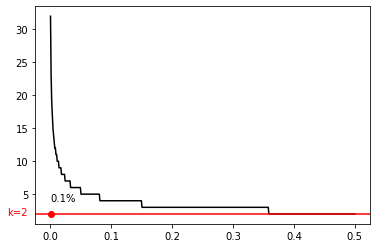
\includegraphics[width=0.5\textwidth]{threshhold-ceil.png}
\end{figure}
 \chapter{Discussion}
I have evaluated two distinct pooling strategies on an ingest consisting of 1560 digital objects. The change rate of the dataset is 32\%, meaning that a third of the objects are expected to be corrupted or changed during the storage in the archive. With an individual testing strategy, 1560 writing operations on the blockchain are needed. The exact gas cost, to persist 1560 SHA256 values is $1560 \cdot 42,368 = 66,094,080$. The cost in USD for that much gas is \$13218.81, assuming a gas price of 50 \acrlong{gwei} and an \acrlong{eth} price of 4000, see Equation \ref{eq:tx-cost}. It is important to denote the operation cost in gas because the gas price is changing in the minute ranging from 30 \acrlong{gwei} up to 60 \acrlong{gwei} and the price of the \acrlong{eth} also fluctuates. With a gas price of 30 \acrlong{gwei}, the operation cost for an ingest of 1560 objects would decrease to \$7931.
Therefore, it is important to be aware of the changing gas prices throughout the day. Gas prices are an indicator on how active the Ethereum network is at the moment, e.g., the gas prices are the lowest in the early morning in Europe when North America is mostly asleep.
I have shown that the amount of costly writing operations can be decreased up to three times utilizing pooled testing. With a two-stage-hierarchical pooling strategy, the amount of writing operations is 520, which results in a total gas cost of $22,031,360$ (\$4406.27).
Although the operation cost was decreased to a third, the cost is still high for a digital archive considering that only a small part of the preservation process is done, persisting fixity information. An operator must decide what is more important to them, the cost, the security or the convenience of their chosen storage-medium for fixity information. 

The proposed implementation of pooled testing, utilizing hash-lists, does not have any method to find out which exact digital object in the pool has changed. On retrieval of a changed object, one must get the SHA256 value from the blockchain and re-compute the SHA256 value of a pool with its respective digital objects. If a mismatch occurs of the two cryptographic hashes, there is no way of defining which exact object in the pool has changed. This is because the information on the integrity of single objects is lost while computing the root hash of a hash-list. Only the resulting root hash matters to guarantee the integrity of the whole pool. The downside of this method is, that one must replace the whole pool with correct copies of the objects every time a corrupt pool is detected. To lower the amount of these data-scrubbing operations, smaller pool sizes are considered in the proposed pooled testing strategies.
In this thesis, I considered bit level error and data manipulation as sources of data change. For legitimate updates, one must either persist a previous version of the object or only persist the SHA256 of the object to be able to re-compute the root hash of the original pool. The updated object than have to be pooled in a new pool with other objects or individually and its hash re-uploaded to the Ethereum blockchain.

The first research question was to find the optimal pool size for the fixity information with respect to two metrics: the first was to minimize the cost and the second was to maximize the efficiency. The two of them were inversely correlated, where to minimize the cost the pool size is N, since there was only one writing transaction on the blockchain when we have only one pool on ingest. On the other hand, a pool size of N is extremely inefficient on retrieval. On retrieval, I have to replace the whole ingest bulk with correct copies if only one object in the pool is corrupt, since I cannot determine which object in the pool got corrupted due to the nature of hash lists. Therefore, I had to also account the number of data scrubbing operations into the optimal pool size, resulting in Equation \ref{eq:expected_data-scrubbing}. The pool size is therefore heavily dependent on the change in the ingest bulk, where if the change rate is high smaller pool sizes are favorable.
For the second research question, I have compared two different approaches for pooled testing. Where the efficiency of both strategies is compared to the efficiency of individual testing. The efficiency of individual testing for sample population of 100 objects where 20 of them are corrupt, meaning that I need 100 writing and additionally 20 data-scrubbing operations during the preservation process. With two stage hierarchical pooling an efficiency of 1.28 can be achieved. In the format-corpus dataset there were just a few file extensions of 90 that were altered and had a change rate greater than 0.0, suggesting that the two-stage strategy was not optimal, since non-volatile files would give been grouped together creating unnecessary traffic on repairing a corrupt pool. Therefore, I have proposed a context-sensitive approach where the inner group change rate of each file extension is considered. Each group in the ingest-bulk is assigned to an own pool with their respective pool size. For instance, in table \ref{tb:efficiency} the file extension PDF has 8 corrupted objects out of 106, which results in a pool size of 8, whereas the XML extension has a much higher corruption rate with an optimal poolside of 2. The context-sensitive approach takes these differences into account and pools homogenous groups, where groups with 0.00 change rate can be grouped with a pool size as large as the inner group. With this method, groups with low change rate can be pooled with large poolside and therefore reduce the cost and increase the efficiency even more than individual testing or two-stage hierarchical pooling.
In the third research question, where I tried to split-off metadata from the digital objects to create a bulk of highly volatile objects and a bulk of stable objects with low change rate, I showed that the approach is worse than with non-split-off metadata. This is because I have to persist the double number of digital objects and the pooling strategies could not compensate for the high number of objects.

The limitations of the strategies proposed in this thesis is the missing data on change rates on digital objects, this is because I would have had to monitor an archive and measure the number of times an object has changed. In this thesis, I have arbitrarily chosen change rates for the objects and their metadata, see Table \ref{tb:split-off}. Future work may propose a method on how to estimate the change rate of an ingest to calculate the real optimal pool size.

The results indicate that the cost for the decentralized fixity storage on the Ethereum blockchain can be reduced, depending on the change rate of the digital objects, by at least 50\%. \chapter{Conclusion}
While the Ethereum blockchain has its limitation regarding the cost, the results of pooled testing showed in this thesis may include the blockchain in future implementations of fixity information storages. This research has shown that the operation cost can be reduced up to a third of cost, but also raises the question if that is enough to establish the Ethereum blockchain as a storage medium for fixity information due to its high cost. While the security and convenience of the Ethereum blockchain stands out, the cost of persisting fixity information for large ingest bulks in digital archives is still high, even after reducing the cost with pooled testing. Operators of digital archives may consider only persisting the fixity of hand-picked digital objects, where security and availability is needed the most, on the blockchain.

A digital archive could deploy the fixity storage on the Ethereum network by setting up an own Ethereum node or by utilizing the developer tools presented in this thesis. After deployment, the operator of the digital archive would be immediately able to persist fixity information on the blockchain after the installation of an Ethereum client of their choice, such as Pythons Web3.py. Due to its minimal requirements, the proposed solution is lightweight and does not require a larger infrastructure to be executed, since the infrastructure to store the fixity information is provided by the Ethereum blockchain.

The optimal pool size for an ingest bulk is dependent on the change rate of its object. For an ingest of N digital objects, the optimal pool size regarding the operation cost is N. With a pool of size N, you only must write once on the blockchain and therefore minimize the cost. But, for a pooling strategy to be efficient, smaller pool sizes have to be chosen to minimize the number of data-scrubbing operations. Therefore, pool sizes from 2 to 10 are favorable, depending on the change rate of the objects. A pool with size 10 is already at the limit of efficiency and can only be considered for non-volatile digital objects which are not expected to change and may only suffer from bit level errors.

With pooled testing, I was able to reduce the operation cost of preserving the fixity information of 1560 digital objects up to a third. The dataset used is the OpenPreserve format-corpus, an openly licensed dataset consisting of various file set and files from creation tools. The cost, utilizing an individual testing strategy was \$13218.81 whereas with a two-stage-hierarchical approach the cost was \$4406.27. In this thesis, it is also shown that the operation cost in USD is not relevant, since it is heavily dependent on the price of gas and the Ether token, the native cryptocurrency of the Ethereum blockchain. In this thesis, I have chosen to present the operation cost in gas which is a constant value and does not change even when the \acrlong{eth} price rises or falls. The presented amount of gas can be converted into USD or any other currency. I have also shown that the efficiency can be improved by a factor of 1.38 with the implementation of context-sensitive pooling. The context-sensitive approach is slightly more efficient than the two-stage-hierarchical pooling due to its consideration of inner group change rates, whereas two-stage-hierarchical pooling only considers a single change rate over the whole ingest bulk.
The third approach, utilizing split-off metadata has shown to have a worse the cost and efficiency compared to with non-split-off metadata. Although, considering with split-off metadata you have the double number of digital objects, the cost of this approach is still almost halved compared to individual testing.

Future work may include the migration of this proposed fixity information storage to another blockchain, a cheaper one. Although you must consider that the price on the established Ethereum network has its security advantages, e.g., denial-of-service attacks only hurts the attacker because of the cost. A good consideration are so-called Layer 2 solutions, which is a term for Ethereum scaling solutions that handle transactions off Ethereum Layer 1 while still taking advantage of the security\footnote{\url{https://ethereum.org/en/layer-2/}}. Layer 2 solutions are considered faster, cheaper, and therefore would be great candidate to enhance the proposed fixity information storage.\\
Future work may also include the estimation of change rates in ingest-bulks to compute the optimal pool size. In this work, I estimated the change rate of the format-corpus dataset by counting the involvement of certain file extensions in Git commits. My suggestion for the estimation is to monitor a digital archive for a certain time interval and count the number of times a certain object has changed. Another interesting method would be, to estimate the change rate of an object based on its file size. If a larger file has a higher chance to experience a bit level error during long term storage.

My contribution to archival science and preservation research was to gather the exact computational effort, in form of gas, needed to operate a decentralized fixity information storage on the Ethereum blockchain. Additionally, I have presented a method to decrease the number of operations and therefore the number of cost relevant transactions needed to operate such an application. With pooled testing, the operation cost of storing the fixity information for 1560 files in format-corpus dataset has been reduced to a third of the cost.
 




\backmatter

\listoffigures 

\listoftables 



\printindex
\printnoidxglossaries
\glsaddall
\bibliographystyle{alpha}
\bibliography{bibliography}
\end{document}